\flushbottom

%% CONTINUE: Needs a lot of work.



%%============================================================================
%%============================================================================
\chapter{First Order Linear Systems of Differential Equations}



We all agree that your theory is crazy, but is it crazy enough?

\begin{flushright}
  - Niels Bohr 
\end{flushright}




%%=============================================================================
\section{Introduction}



%% CONTINUE: Motivating example.


In this chapter we consider first order linear systems of differential 
equations.  That is, we consider equations of the form,
\begin{gather*}
  \mathbf{x}'(t) = \mathbf{A} \mathbf{x}(t) + \mathbf{f}(t),
  \\
  \mathbf{x}(t) = \begin{pmatrix} x_1(t) \\ \vdots \\ x_n(t) \end{pmatrix},
  \qquad
  \mathbf{A} = 
  \begin{pmatrix}
    a_{11}       & a_{12}     & \ldots        &a_{1n} \\
    a_{21}       & a_{22}     & \ldots        &a_{2n} \\
    \vdots          & \vdots        & \ddots        & \vdots \\
    a_{n1}       & a_{n2}     & \ldots        &a_{nn}
  \end{pmatrix}.
\end{gather*}
Initially we will consider the homogeneous problem, 
$\mathbf{x}'(t) = \mathbf{A} \mathbf{x}(t)$.  (Later we will find particular solutions with 
variation of parameters.)  The best way to solve these equations is through
the use of the matrix exponential.  Unfortunately, using the matrix 
exponential requires knowledge of the Jordan canonical form and matrix 
functions.  Fortunately, we can solve a certain class of problems using 
only the concepts of eigenvalues and eigenvectors of a matrix.  We present
this simple method in the next section.  In the following section
we will take a detour into
matrix theory to cover Jordan canonical form and its applications.  Then
we will be able to solve the general case.









%%=============================================================================
\section{Using Eigenvalues and Eigenvectors to find Homogeneous Solutions}







If you have forgotten what eigenvalues and eigenvectors are and how to compute
them, go find
a book on linear algebra and spend a few minutes re-aquainting yourself 
with the rudimentary material.
%% CONTINUE: add linear algebra to the book.


Recall that the single differential equation $x'(t) = A x$ has the general
solution $x = c \e^{A t}$.  Maybe the system of differential equations 
\begin{equation}
  \label{eq:x'=Ax}
  \mathbf{x}'(t) = \mathbf{A} \mathbf{x}(t)
\end{equation}
has similiar solutions.  Perhaps it has a solution
of the form $\mathbf{x}(t) = \boldsymbol{\xi} \e^{\lambda t}$ for some constant vector $\boldsymbol{\xi}$ and 
some value $\lambda$.  Let's substitute this into the differential equation
and see what happens.
\begin{gather*}
  \mathbf{x}'(t) = \mathbf{A} \mathbf{x}(t)
  \\
  \boldsymbol{\xi} \lambda \e^{\lambda t} = \mathbf{A} \boldsymbol{\xi} \e^{\lambda t}
  \\
  \mathbf{A} \boldsymbol{\xi} = \lambda \boldsymbol{\xi}
\end{gather*}
We see that if $\lambda$ is an eigenvalue of $\mathbf{A}$ with eigenvector $\boldsymbol{\xi}$
then $\mathbf{x}(t) = \boldsymbol{\xi} \e^{\lambda t}$ satisfies the differential equation.  Since 
the differential equation is linear, $c \boldsymbol{\xi} \e^{\lambda t}$ is a solution.

Suppose that the $n \times n$ matrix $\mathbf{A}$ has the eigenvalues $\{ \lambda_k \}$ 
with a complete
set of linearly independent eigenvectors $\{ \boldsymbol{\xi}_k \}$.  Then each of
$\boldsymbol{\xi}_k \e^{\lambda_k t}$ is a homogeneous solution of Equation~\ref{eq:x'=Ax}.
We note that each of these solutions is linearly independent.  Without
any kind of justification I will tell you that the general solution of
the differential equation is a linear combination of these $n$ linearly 
independent solutions.
%% CONTINUE



\begin{Result}
  Suppose that the $n \times n$ matrix $\mathbf{A}$ has the eigenvalues $\{ \lambda_k \}$ 
  with a complete set of linearly independent eigenvectors $\{ \boldsymbol{\xi}_k \}$.
  The system of differential equations,
  \[
  \mathbf{x}'(t) = \mathbf{A} \mathbf{x}(t),
  \]
  has the general solution,
  \[
  \mathbf{x}(t) = \sum_{k = 1}^n c_k \boldsymbol{\xi}_k \e^{\lambda_k t}
  \]
\end{Result}




%% CONTINUE WRITE MORE





\begin{Example}[mathematica/ode/systems/systems.nb]
  Find the solution of the following initial value problem.
  Describe the behavior of the solution as $t \to \infty$.
  \[
  \mathbf{x}' = \mathbf{A} x \equiv
  \begin{pmatrix}
    -2 & 1\\
    -5 & 4
  \end{pmatrix} 
  \mathbf{x}, \quad 
  \mathbf{x}(0) = \mathbf{x}_0 \equiv
  \begin{pmatrix}
    1\\
    3
  \end{pmatrix}
  \]

  The matrix has the distinct eigenvalues $\lambda_1 = -1$, $\lambda_2 = 3$.  The 
  corresponding eigenvectors are 
  \[
  \mathbf{x}_1 = \begin{pmatrix} 1 \\ 1 \end{pmatrix}, \quad
  \mathbf{x}_2 = \begin{pmatrix} 1 \\ 5 \end{pmatrix}.
  \]
  The general solution of the system of differential equations is
  \[
  \mathbf{x} = 
  c_1 \begin{pmatrix} 1 \\ 1 \end{pmatrix} \e^{-t}
  + c_2 \begin{pmatrix} 1 \\ 5 \end{pmatrix} \e^{3 t}.
  \]
  We apply the initial condition to determine the constants.
  \begin{gather*}
    \begin{pmatrix}
      1 & 1 \\
      1 & 5
    \end{pmatrix}
    \begin{pmatrix}
      c_1 \\
      c_2
    \end{pmatrix}
    =
    \begin{pmatrix}
      1 \\
      3
    \end{pmatrix} \\
    c_1 = \frac{1}{2}, \quad c_2 = \frac{1}{2}
  \end{gather*}
  The solution subject to the initial condition is
  \[
  \boxed{
    \mathbf{x} = 
    \frac{1}{2} \begin{pmatrix} 1 \\ 1 \end{pmatrix} \e^{-t}
    + \frac{1}{2} \begin{pmatrix} 1 \\ 5 \end{pmatrix} \e^{3 t}
    }
  \]
  For large $t$, the solution looks like
  \[
  \mathbf{x} \approx \frac{1}{2} \begin{pmatrix} 1 \\ 5 \end{pmatrix} \e^{3 t}.
  \]
  Both coordinates tend to infinity.

  Figure~\ref{x_2154x} shows some homogeneous solutions in the phase plane.
  \begin{figure}[tb!]
    \begin{center}
      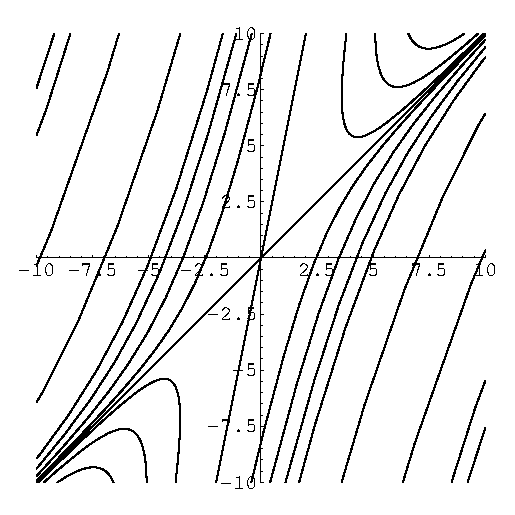
\includegraphics[width=0.4\textwidth]{ode/systems/x_2154x}
    \end{center}
    \caption{Homogeneous solutions in the phase plane.}
    \label{x_2154x}
  \end{figure}
\end{Example}











\begin{Example}[mathematica/ode/systems/systems.nb]
  Find the solution of the following initial value problem.
  Describe the behavior of the solution as $t \to \infty$.
  \[
  \mathbf{x}' = \mathbf{A} x \equiv
  \begin{pmatrix}
    1 & 1 & 2 \\
    0 & 2 & 2 \\
    -1 & 1 & 3
  \end{pmatrix} 
  \mathbf{x}, \quad 
  \mathbf{x}(0) = \mathbf{x}_0 \equiv
  \begin{pmatrix}
    2 \\
    0 \\
    1
  \end{pmatrix}
  \]

  The matrix has the distinct eigenvalues $\lambda_1 = 1$, $\lambda_2 = 2$, $\lambda_3 = 3$.  The 
  corresponding eigenvectors are 
  \[
  \mathbf{x}_1 = \begin{pmatrix} 0 \\ -2 \\ 1 \end{pmatrix}, \quad
  \mathbf{x}_2 = \begin{pmatrix} 1 \\ 1 \\ 0 \end{pmatrix}, \quad
  \mathbf{x}_3 = \begin{pmatrix} 2 \\ 2 \\ 1 \end{pmatrix}.
  \]
  The general solution of the system of differential equations is
  \[
  \mathbf{x} = 
  c_1 \begin{pmatrix} 0 \\ -2 \\ 1 \end{pmatrix} \e^t
  + c_2 \begin{pmatrix} 1 \\ 1 \\ 0 \end{pmatrix} \e^{2 t}
  + c_3 \begin{pmatrix} 2 \\ 2 \\ 1 \end{pmatrix} \e^{3 t}.
  \]
  We apply the initial condition to determine the constants.
  \begin{gather*}
    \begin{pmatrix}
      0 & 1 & 2 \\
      -2 & 1 & 2 \\
      1 & 0 & 1
    \end{pmatrix}
    \begin{pmatrix}
      c_1 \\
      c_2 \\
      c_3
    \end{pmatrix}
    =
    \begin{pmatrix}
      2 \\
      0 \\
      1
    \end{pmatrix} \\
    c_1 = 1, \quad c_2 = 2, \quad c_3 = 0
  \end{gather*}
  The solution subject to the initial condition is
  \[
  \boxed{
    \mathbf{x} = 
    \begin{pmatrix} 0 \\ -2 \\ 1 \end{pmatrix} \e^t
    + 2 \begin{pmatrix} 1 \\ 1 \\ 0 \end{pmatrix} \e^{2 t}.
    }
  \]
  As $t \to \infty$, all coordinates tend to infinity.
\end{Example}







\begin{Exercise}[mathematica/ode/systems/systems.nb]
  \label{exercise x'=(1-51-3)x t-infinity}
  Find the solution of the following initial value problem.
  Describe the behavior of the solution as $t \to \infty$.
  \[
  \mathbf{x}' = \mathbf{A} x \equiv
  \begin{pmatrix}
    1 & -5 \\
    1 & -3
  \end{pmatrix} 
  \mathbf{x}, \quad 
  \mathbf{x}(0) = \mathbf{x}_0 \equiv
  \begin{pmatrix}
    1 \\
    1
  \end{pmatrix}
  \]

  \hintsolution{x'=(1-51-3)x t-infinity}
\end{Exercise}




\begin{Exercise}[mathematica/ode/systems/systems.nb]
  \label{exercise x'=(-3021-10-2-10)x t-infinity}
  Find the solution of the following initial value problem.
  Describe the behavior of the solution as $t \to \infty$.
  \[
  \mathbf{x}' = \mathbf{A} x \equiv
  \begin{pmatrix}
    -3 & 0 & 2 \\
    1 & -1 & 0 \\
    -2 & -1 & 0
  \end{pmatrix} 
  \mathbf{x}, \quad 
  \mathbf{x}(0) = \mathbf{x}_0 \equiv
  \begin{pmatrix}
    1 \\
    0 \\
    0
  \end{pmatrix}
  \]

  \hintsolution{x'=(-3021-10-2-10)x t-infinity}
\end{Exercise}




%% Use the matrix form of the method of variation of parameters to find the 
\begin{Exercise}
  \label{exercise dxdt=4284x+t3t2}
  Use the matrix form of the method of variation of parameters to find the 
  general solution of
  \[
  \frac{\dd \mathbf{x}}{\dd t} = 
  \begin{pmatrix}
    4 & -2 \\
    8 & -4
  \end{pmatrix}
  \mathbf{x} + 
  \begin{pmatrix}
    t^{-3} \\
    -t^{-2}
  \end{pmatrix},
  \quad t > 0.
  \]

  \hintsolution{dxdt=4284x+t3t2}
\end{Exercise}








%%=============================================================================
\section{Matrices and Jordan Canonical Form} 


%% CONTINUE: convergence
\paragraph{Functions of Square Matrices.}
Consider a function $f(x)$ with a Taylor series.
\[
f(x) = \sum_{n = 0}^\infty \frac{f^{(n)}(0)}{n!} x^n
\]
We can define the function to take square matrices as arguments.
The function of the square matrix $\mathbf{A}$ is defined in terms of the 
Taylor series.
\[
f(\mathbf{A}) = \sum_{n = 0}^\infty \frac{f^{(n)}(0)}{n!} \mathbf{A}^n
\]
(Note that this definition is usually not the most convenient method
for computing a function of a matrix.  Use the Jordan canonical form for
that.)






\paragraph{Eigenvalues and Eigenvectors.}
Consider a square matrix $\mathbf{A}$.
A nonzero vector $\mathbf{x}$ is an \textit{eigenvector} of the matrix with 
\textit{eigenvalue} $\lambda$ if 
\[
\mathbf{A} \mathbf{x} = \lambda \mathbf{x}.
\]
Note that we can write this equation as
\[
(\mathbf{A} - \lambda \mathbf{I}) \mathbf{x} = \mathbf{0}.
\]
This equation has solutions for nonzero $\mathbf{x}$ if and only if 
$\mathbf{A} - \lambda \mathbf{I}$ is singular, ($\det(\mathbf{A} - \lambda \mathbf{I}) = 0$).
We define the \textit{characteristic polynomial} of the matrix $\chi(\lambda)$ as 
this determinant.
\[
\chi(\lambda) = \det(\mathbf{A} - \lambda \mathbf{I})
\]
The roots of the characteristic polynomial are the eigenvalues of the matrix.
The eigenvectors of distinct eigenvalues are linearly independent.  
Thus if a matrix has distinct eigenvalues, the eigenvectors form a basis.

If $\lambda$ is a root of $\chi(\lambda)$ of multiplicity $m$ then there 
are up to $m$ linearly independent eigenvectors corresponding to that 
eigenvalue.  That is, it has from $1$ to $m$ eigenvectors.





\paragraph{Diagonalizing Matrices.}
Consider an $n \times n$ matrix $\mathbf{A}$ that has a complete set of $n$ 
linearly independent eigenvectors.  $\mathbf{A}$ may or may not have distinct
eigenvalues.  Consider the matrix $\mathbf{S}$ with eigenvectors as columns.
\[
\mathbf{S} =
\begin{pmatrix}
  \mathbf{x}_1 & \mathbf{x}_2 & \cdots & \mathbf{x}_n 
\end{pmatrix}
\]
$\mathbf{A}$ is diagonalized by the similarity transformation:
\[
\boldsymbol{\Lambda} = \mathbf{S}^{-1} \mathbf{A} \mathbf{S}.
\]
$\boldsymbol{\Lambda}$ is a diagonal matrix with the eigenvalues of $\mathbf{A}$ as the 
diagonal elements.  Furthermore, the $k^{\mathrm{th}}$ diagonal element
is $\lambda_k$, the eigenvalue corresponding to the the eigenvector,
$\mathbf{x}_k$.






\paragraph{Generalized Eigenvectors.}
A vector $\mathbf{x}_k$ is a \textit{generalized eigenvector of rank} $k$ if
\[
(\mathbf{A} - \lambda \mathbf{I})^k \mathbf{x}_k = \mathbf{0} \quad \mathrm{but} \quad
(\mathbf{A} - \lambda \mathbf{I})^{k-1} \mathbf{x}_{k} \neq \mathbf{0}.
\]
Eigenvectors are generalized eigenvectors of rank 1.
An $n \times n$ matrix has $n$ linearly independent generalized eigenvectors.
A \textit{chain} of generalized eigenvectors generated by the rank $m$ 
generalized eigenvector $\mathbf{x}_m$ is the set:
$\{ \mathbf{x}_1, \mathbf{x}_2, \ldots, \mathbf{x}_m \}$,
where 
\[
\mathbf{x}_k = (\mathbf{A} - \lambda \mathbf{I}) \mathbf{x}_{k+1}, \quad \mathrm{for} \quad
k = m-1, \ldots, 1.
\]


\paragraph{Computing Generalized Eigenvectors.}

Let $\lambda$ be an eigenvalue of multiplicity $m$.  Let $n$ be the smallest
integer such that
\[
\rank \left( \nullspace \left( (A - \lambda I)^n \right) \right) = m.
\]
Let $N_k$ denote the number of eigenvalues of rank $k$.  These 
have the value:
\[
N_k = \rank \left( \nullspace \left( (A - \lambda I)^k \right) \right)
- \rank \left( \nullspace \left( (A - \lambda I)^{k-1} \right) \right).
\]

One can compute the generalized eigenvectors of a matrix by looping 
through the following three steps until all the the $N_k$ are zero:
\begin{enumerate}
  %%
\item Select the largest $k$ for which $N_k$ is positive.  Find a 
  generalized eigenvector $\mathbf{x}_k$ of rank $k$ which is linearly independent 
  of all the generalized eigenvectors found thus far.  
  %%
\item From $\mathbf{x}_k$ generate the 
  chain of eigenvectors $\{\mathbf{x}_1, \mathbf{x}_2, \ldots, \mathbf{x}_k\}$.  Add this 
  chain to the known generalized eigenvectors.
  %%
\item
  Decrement each positive $N_k$ by one.
\end{enumerate}


\begin{Example}
  \label{example_gen_eigenvec_111}
  Consider the matrix
  \[
  \mathbf{A} = 
  \begin{pmatrix}
    1 & 1 & 1 \\
    2 & 1 & -1 \\
    -3 & 2 & 4 
  \end{pmatrix}.
  \]
  The characteristic polynomial of the matrix is
  \begin{align*}
    \chi(\lambda)
    &= \begin{vmatrix}
      1 - \lambda  & 1             & 1 \\
      2               & 1 - \lambda        & -1 \\
      -3              & 2             & 4 - \lambda
    \end{vmatrix} \\
    &= (1-\lambda)^2 (4 - \lambda) + 3 + 4 +3 (1-\lambda)
    -2 (4-\lambda) + 2 (1-\lambda) \\
    &= - (\lambda - 2)^3.
  \end{align*}
  Thus we see that $\lambda = 2$ is an eigenvalue of multiplicity 3.  
  $\mathbf{A} - 2 \mathbf{I}$ is
  \[
  \mathbf{A}  - 2 \mathbf{I}
  =
  \begin{pmatrix}
    -1 & 1 & 1 \\
    2 & -1 & -1 \\
    -3 & 2 & 2 
  \end{pmatrix}
  \]
  The rank of the nullspace space of $\mathbf{A} - 2 \mathbf{I}$ is less than 3.
  \[
  (\mathbf{A}  - 2 \mathbf{I})^2
  =
  \begin{pmatrix}
    0 & 0 & 0 \\
    -1 & 1 & 1 \\
    1 & -1 & -1 
  \end{pmatrix}
  \]
  The rank of $\nullspace((\mathbf{A} - 2 \mathbf{I})^2)$ is less than 3 as well, so we have to 
  take one more step.
  \[
  (\mathbf{A}  - 2 \mathbf{I})^3
  =
  \begin{pmatrix}
    0 & 0 & 0 \\
    0 & 0 & 0 \\
    0 & 0 & 0
  \end{pmatrix}
  \]
  The rank of $\nullspace((\mathbf{A} - 2 \mathbf{I})^3)$ is 3.  Thus there are generalized
  eigenvectors of ranks 1, 2 and 3.  The generalized eigenvector of rank 3
  satisfies:
  \begin{gather*}
    (\mathbf{A}  - 2 \mathbf{I})^3 \mathbf{x}_{3} = \mathbf{0} \\
    \begin{pmatrix}
      0 & 0 & 0 \\
      0 & 0 & 0 \\
      0 & 0 & 0
    \end{pmatrix}
    \mathbf{x}_{3} = \mathbf{0}
  \end{gather*}
  We choose the solution
  \[
  \mathbf{x}_{3} = 
  \begin{pmatrix}
    1 \\
    0 \\
    0
  \end{pmatrix}.
  \]
  Now to compute the chain generated by $\mathbf{x}_{3}$.
  \begin{gather*}
    \mathbf{x}_{2} = (\mathbf{A} - 2 \mathbf{I}) \mathbf{x}_{3} = 
    \begin{pmatrix}
      -1 \\
      2 \\
      -3
    \end{pmatrix} \\
    \mathbf{x}_{1} = (\mathbf{A} - 2 \mathbf{I}) \mathbf{x}_{2} = 
    \begin{pmatrix}
      0 \\
      -1 \\
      1
    \end{pmatrix}
  \end{gather*}

  Thus a set of generalized eigenvectors corresponding to the eigenvalue 
  $\lambda = 2$ are
  \[
  \boxed{
    \mathbf{x}_{1} =
    \begin{pmatrix}
      0 \\
      -1 \\
      1
    \end{pmatrix},
    \quad
    \mathbf{x}_{2} =
    \begin{pmatrix}
      -1 \\
      2 \\
      -3
    \end{pmatrix},
    \quad
    \mathbf{x}_{3} = 
    \begin{pmatrix}
      1 \\
      0 \\
      0
    \end{pmatrix}.
    }
  \]
\end{Example}





\paragraph{Jordan Block.}
A Jordan block is a square matrix which has the constant, $\lambda$,
on the diagonal and ones on the first super-diagonal:
\[
\begin{pmatrix}
  \lambda      & 1     & 0     &\cdots     & 0     & 0     \\
  0       &\lambda& 1  &\cdots & 0         & 0     \\
  0       & 0     &\lambda&\ddots & 0      & 0     \\
  \vdots      &\vdots     &\ddots &\ddots &\ddots &\vdots \\
  0       & 0     & 0     &\ddots     &\lambda& 1  \\
  0       & 0     & 0     &\cdots     & 0     &\lambda
\end{pmatrix}
\]



\paragraph{Jordan Canonical Form.}
A matrix $\mathbf{J}$ is in Jordan canonical form if all the elements are zero 
except for Jordan blocks $\mathbf{J}_k$ along the diagonal.
\[
\mathbf{J} = 
\begin{pmatrix}
  \mathbf{J}_1  & \mathbf{0}  &\cdots     & \mathbf{0}  & \mathbf{0} \\
  \mathbf{0}    &\mathbf{J}_2 &\ddots     & \mathbf{0}  & \mathbf{0} \\
  \vdots      &\ddots     &\ddots &\ddots &\vdots\\
  \mathbf{0}    & \mathbf{0}  &\ddots     & \mathbf{J}_{n-1}& \mathbf{0} \\
  \mathbf{0}    & \mathbf{0}  &\cdots     & \mathbf{0}  & \mathbf{J}_n
\end{pmatrix}
\]
The Jordan canonical form of a matrix is obtained with the similarity
transformation:
\[
\mathbf{J} = \mathbf{S}^{-1} \mathbf{A} \mathbf{S},
\]
where $\mathbf{S}$ is the matrix of the generalized eigenvectors of $\mathbf{A}$ and
the generalized eigenvectors are grouped in chains.






\begin{Example}
  \label{example_jordan_111}
  Again consider the matrix
  \[
  \mathbf{A} = 
  \begin{pmatrix}
    1 & 1 & 1 \\
    2 & 1 & -1 \\
    -3 & 2 & 4 
  \end{pmatrix}.
  \]
  Since $\lambda = 2$ is an eigenvalue of multiplicity 3, the Jordan canonical
  form of the matrix is
  \[
  \mathbf{J} = 
  \begin{pmatrix}
    2 & 1 & 0 \\
    0 & 2 & 1 \\
    0 & 0 & 2 
  \end{pmatrix}.
  \]
  In Example~\ref{example_gen_eigenvec_111} we found the generalized 
  eigenvectors of
  $\mathbf{A}$.  We define the matrix with generalized eigenvectors as columns:
  \[
  \mathbf{S} = 
  \begin{pmatrix}
    0 & -1 & 1 \\
    -1 & 2 & 0 \\
    1 & -3 & 0 
  \end{pmatrix}.
  \]
  We can verify that $\mathbf{J} = \mathbf{S}^{-1} \mathbf{A} \mathbf{S}$.
  \begin{align*}
    \mathbf{J}    &= \mathbf{S}^{-1} \mathbf{A} \mathbf{S} \\
    &=      \begin{pmatrix}
      0 & -3 & -2 \\
      0 & -1 & -1 \\
      1 & -1 & -1 
    \end{pmatrix}
    \begin{pmatrix}
      1 & 1 & 1 \\
      2 & 1 & -1 \\
      -3 & 2 & 4 
    \end{pmatrix}
    \begin{pmatrix}
      0 & -1 & 1 \\
      -1 & 2 & 0 \\
      1 & -3 & 0 
    \end{pmatrix} \\
    &=      \begin{pmatrix}
      2 & 1 & 0 \\
      0 & 2 & 1 \\
      0 & 0 & 2 
    \end{pmatrix}
  \end{align*}
\end{Example}





%% CONTINUE: Cayley Hamilton -> polynomial



\paragraph{Functions of Matrices in Jordan Canonical Form.}
The function of an $n \times n$ Jordan block is the upper-triangular matrix:
\[
f(\mathbf{J}_k) = 
\begin{pmatrix}
  f(\lambda)& \frac{f'(\lambda)}{1!}& \frac{f''(\lambda)}{2!} &\cdots& 
  \frac{f^{(n-2)}(\lambda)}{(n-2)!}& \frac{f^{(n-1)}(\lambda)}{(n-1)!}\\
  0       &f(\lambda)& \frac{f'(\lambda)}{1!}&\cdots & 
  \frac{f^{(n-3)}(\lambda)}{(n-3)!}    & 
  \frac{f^{(n-2)}(\lambda)}{(n-2)!}\\
  0       & 0     &f(\lambda)&\ddots & \frac{f^{(n-4)}(\lambda)}{(n-4)!}        & 
  \frac{f^{(n-3)}(\lambda)}{(n-3)!}    \\
  \vdots      &\vdots     &\ddots &\ddots &\ddots &\vdots \\
  0       & 0     & 0     &\ddots     &f(\lambda)& \frac{f'(\lambda)}{1!}\\
  0       & 0     & 0     &\cdots     & 0     &f(\lambda)
\end{pmatrix}
\]
The function of a matrix in Jordan canonical form is
\[
f(\mathbf{J}) = 
\begin{pmatrix}
  f(\mathbf{J}_1)& \mathbf{0} &\cdots     & \mathbf{0}  & \mathbf{0} \\
  \mathbf{0}    &f(\mathbf{J}_2)&\ddots   & \mathbf{0}  & \mathbf{0} \\
  \vdots      &\ddots     &\ddots &\ddots &\vdots\\
  \mathbf{0}    & \mathbf{0}  &\ddots     & f(\mathbf{J}_{n-1})& \mathbf{0} \\
  \mathbf{0}    & \mathbf{0}  &\cdots     & \mathbf{0}  & f(\mathbf{J}_n)
\end{pmatrix}
\]
The Jordan canonical form of a matrix satisfies:
\[
f(\mathbf{J}) = \mathbf{S}^{-1} f(\mathbf{A}) \mathbf{S},
\]
where $\mathbf{S}$ is the matrix of the generalized eigenvectors of $\mathbf{A}$.
This gives us a convenient method for computing functions of matrices.





\begin{Example}
  \label{example_eAt_111}
  Consider the matrix exponential function $\e^{\mathbf{A}}$ for our old friend:
  \[
  \mathbf{A} = 
  \begin{pmatrix}
    1 & 1 & 1 \\
    2 & 1 & -1 \\
    -3 & 2 & 4 
  \end{pmatrix}.
  \]
  In Example~\ref{example_jordan_111} we showed that the Jordan canonical
  form of the matrix is
  \[
  \mathbf{J} = 
  \begin{pmatrix}
    2 & 1 & 0 \\
    0 & 2 & 1 \\
    0 & 0 & 2 
  \end{pmatrix}.
  \]
  Since all the derivatives of $\e^\lambda$ are just $\e^\lambda$, 
  it is especially easy to compute $\e^{\mathbf{J}}$.
  \[
  \e^{\mathbf{J}} = 
  \begin{pmatrix}
    \e^2 & \e^2 & \e^2/2 \\
    0 & \e^2 & \e^2 \\
    0 & 0 & \e^2 
  \end{pmatrix}
  \]
  We find $\e^{\mathbf{A}}$ with a similarity transformation of $\e^{\mathbf{J}}$.
  We use the matrix of generalized eigenvectors found in 
  Example~\ref{example_jordan_111}.
  \begin{gather*}
    \e^{\mathbf{A}} = \mathbf{S} \e^{\mathbf{J}} \mathbf{S}^{-1} \\
    \e^{\mathbf{A}} =     \begin{pmatrix}
      0 & -1 & 1 \\
      -1 & 2 & 0 \\
      1 & -3 & 0 
    \end{pmatrix} 
    \begin{pmatrix}
      \e^2 & \e^2 & \e^2/2 \\
      0 & \e^2 & \e^2 \\
      0 & 0 & \e^2 
    \end{pmatrix}
    \begin{pmatrix}
      0 & -3 & -2 \\
      0 & -1 & -1 \\
      1 & -1 & -1 
    \end{pmatrix} \\
    \boxed{
      \e^{\mathbf{A}} =     \begin{pmatrix}
        0 & 2 & 2 \\
        3 & 1 & -1 \\
        -5 & 3 & 5
      \end{pmatrix} \frac{\e^2}{2}
      }
  \end{gather*}
\end{Example}










%%=============================================================================
\section{Using the Matrix Exponential}





The homogeneous differential equation
\[
\mathbf{x}'(t) = \mathbf{A} \mathbf{x}(t)
\]
has the solution
\[
\mathbf{x}(t) = \e^{\mathbf{A} t} \mathbf{c}
\]
where $\mathbf{c}$ is a vector of constants.  The solution subject to the initial
condition, $\mathbf{x}(t_0) = \mathbf{x}_0$ is
\[
\mathbf{x}(t) = \e^{\mathbf{A} (t - t_0)} \mathbf{x}_0.
\]

The homogeneous differential equation
\[
\mathbf{x}'(t) = \frac{1}{t} \mathbf{A} \mathbf{x}(t)
\]
has the solution
\[
\mathbf{x}(t) = t^{\mathbf{A}} \mathbf{c} \equiv \e^{\mathbf{A} \Log t} \mathbf{c},
\]
where $\mathbf{c}$ is a vector of constants.  The solution subject to the initial
condition, $\mathbf{x}(t_0) = \mathbf{x}_0$ is
\[
\mathbf{x}(t) = \left( \frac{t}{t_0} \right)^{\mathbf{A}} \mathbf{x}_0
\equiv \e^{\mathbf{A} \Log(t / t_0)} \mathbf{x}_0.
\]

The inhomogeneous problem
\[
\mathbf{x}'(t) = \mathbf{A} \mathbf{x}(t) + \mathbf{f}(t), \quad \mathbf{x}(t_0) = \mathbf{x}_0
\]
has the solution
\[
\mathbf{x}(t) = \e^{\mathbf{A} (t - t_0)} \mathbf{x}_0 
+ \e^{\mathbf{A} t} \int_{t_0}^t \e^{-\mathbf{A} \tau} \mathbf{f}(\tau) \,\dd \tau.
\]










\begin{Example}
  Consider the system
  \[
  \frac{\dd \mathbf{x}}{\dd t} = 
  \begin{pmatrix}
    1 & 1 & 1 \\
    2 & 1 & -1 \\
    -3 & 2 & 4 
  \end{pmatrix}
  \mathbf{x}.
  \]
  The general solution of the system of differential equations is
  \[
  \mathbf{x}(t) = \e^{\mathbf{A} t} \mathbf{c}.
  \]
  In Example~\ref{example_eAt_111} we found $\e^{\mathbf{A}}$.  $\mathbf{A} t$ is just
  a constant times $\mathbf{A}$. The eigenvalues
  of $\mathbf{A} t$ are $\{\lambda_k t\}$ where $\{\lambda_k\}$ are the 
  eigenvalues of $\mathbf{A}$.  The generalized eigenvectors of $\mathbf{A} t$ are the
  same as those of $\mathbf{A}$.  

  Consider $\e^{\mathbf{J} t}$.  The derivatives of $f(\lambda) = \e^{\lambda t}$ 
  are $f'(\lambda) = t \e^{\lambda t}$ and $f''(\lambda) = t^2 \e^{\lambda t}$.
  Thus we have
  \begin{gather*}
    \e^{\mathbf{J} t} = 
    \begin{pmatrix}
      \e^{2 t} & t \e^{2 t} & t^2 \e^{2 t} / 2 \\
      0 & \e^{2 t} & t \e^{2 t} \\
      0 & 0 & \e^{2 t}
    \end{pmatrix} \\
    \e^{\mathbf{J} t} = 
    \begin{pmatrix}
      1 & t & t^2 / 2 \\
      0 & 1 & t \\
      0 & 0 & 1
    \end{pmatrix} \e^{2 t}
  \end{gather*}
  We find $\e^{A t}$ with a similarity transformation.
  \begin{gather*}
    \e^{\mathbf{A} t} = \mathbf{S} \e^{\mathbf{J} t} \mathbf{S}^{-1} \\
    \e^{\mathbf{A} t} =   \begin{pmatrix}
      0 & -1 & 1 \\
      -1 & 2 & 0 \\
      1 & -3 & 0 
    \end{pmatrix} 
    \begin{pmatrix}
      1 & t & t^2 / 2 \\
      0 & 1 & t \\
      0 & 0 & 1
    \end{pmatrix} \e^{2 t}
    \begin{pmatrix}
      0 & -3 & -2 \\
      0 & -1 & -1 \\
      1 & -1 & -1 
    \end{pmatrix} \\
    \e^{\mathbf{A} t} = 
    \begin{pmatrix}
      1-t & t & t \\
      2 t-t^2 / 2 & 1 - t + t^2 / 2 & -t + t^2 / 2 \\
      -3 t + t^2 / 2 & 2 t - t^2 / 2 & 1 + 2 t - t^2 / 2 
    \end{pmatrix}
    \e^{2 t}
  \end{gather*}
  The solution of the system of differential equations is
  \[
  \boxed{
    \mathbf{x}(t) = 
    \left(
      c_1
      \begin{pmatrix}
        1-t \\
        2 t-t^2 / 2 \\
        -3 t + t^2 / 2
      \end{pmatrix}
      + c_2 
      \begin{pmatrix}
        t \\
        1 - t + t^2 / 2 \\
        2 t - t^2 / 2
      \end{pmatrix}
      + c_3
      \begin{pmatrix}
        t \\
        -t + t^2 / 2 \\
        1 + 2 t - t^2 / 2 
      \end{pmatrix}
    \right) \e^{2 t}
    }
  \]
\end{Example}











\begin{Example}
  Consider the Euler equation system
  \[
  \frac{\dd \mathbf{x}}{\dd t} 
  = \frac{1}{t} \mathbf{A} \mathbf{x}
  \equiv \frac{1}{t} 
  \begin{pmatrix}
    1 & 0 \\
    1 & 1
  \end{pmatrix}
  \mathbf{x}.
  \]
  The solution is $\mathbf{x}(t) = t^{\mathbf{A}} \mathbf{c}$.
  Note that $\mathbf{A}$ is almost in Jordan canonical form. It has a one on 
  the sub-diagonal instead of the super-diagonal.  It is clear that
  a function of $\mathbf{A}$ is defined
  \[
  f(\mathbf{A}) = 
  \begin{pmatrix}
    f(1) & 0 \\
    f'(1) & f(1)
  \end{pmatrix}.
  \]
  The function $f(\lambda) = t^\lambda$ has the derivative
  $f'(\lambda) = t^\lambda \log t$.  Thus the solution of the system is
  \[
  \boxed{
    \mathbf{x}(t) = 
    \begin{pmatrix}
      t & 0 \\
      t \log t & t
    \end{pmatrix}
    \begin{pmatrix}
      c_1 \\
      c_2
    \end{pmatrix}
    =
    c_1 
    \begin{pmatrix}
      t \\
      t \log t
    \end{pmatrix}
    + c_2 
    \begin{pmatrix}
      0 \\
      t
    \end{pmatrix}
    }
  \]
\end{Example}









\begin{Example}
  Consider an inhomogeneous system of differential equations.
  \[
  \frac{\dd \mathbf{x}}{\dd t} 
  = \mathbf{A} \mathbf{x} + \mathbf{f}(t)
  \equiv
  \begin{pmatrix}
    4 & -2 \\
    8 & -4
  \end{pmatrix}
  \mathbf{x} + 
  \begin{pmatrix}
    t^{-3} \\
    -t^{-2}
  \end{pmatrix},
  \quad t > 0.
  \]
  The general solution is 
  \[
  \mathbf{x}(t) = \e^{\mathbf{A} t} \mathbf{c} + \e^{\mathbf{A} t} \int \e^{-\mathbf{A} t} f(t) \,\dd t.
  \]
  First we find homogeneous solutions.  The characteristic equation for 
  the matrix is
  \[
  \chi(\lambda) = 
  \begin{vmatrix}
    4 - \lambda & -2 \\
    8 & -4 - \lambda
  \end{vmatrix} =
  \lambda^2 = 0
  \]
  $\lambda = 0$ is an eigenvalue of multiplicity 2.  
  Thus the Jordan canonical form of the matrix is 
  \[
  \mathbf{J} = \begin{pmatrix}
    0 & 1 \\
    0 & 0
  \end{pmatrix}.
  \]

  Since $\rank(\nullspace(\mathbf{A} - 0 \mathbf{I})) = 1$ there is only one eigenvector.  
  A generalized eigenvector of rank 2 satisfies
  \begin{gather*}
    (\mathbf{A} - 0 \mathbf{I})^2 \mathbf{x}_2 = \mathbf{0} \\
    %%
    \begin{pmatrix}
      0 & 0 \\
      0 & 0
    \end{pmatrix}
    \mathbf{x}_2 = \mathbf{0} 
  \end{gather*}
  We choose
  \[
  \mathbf{x}_2 = \begin{pmatrix}
    1 \\
    0
  \end{pmatrix}
  \]
  Now we generate the chain from $\mathbf{x}_2$.
  \[
  \mathbf{x}_1 = (\mathbf{A} - 0 \mathbf{I}) \mathbf{x}_2 = 
  \begin{pmatrix}
    4 \\
    8
  \end{pmatrix}
  \]
  We define the matrix of generalized eigenvectors $\mathbf{S}$.
  \[
  \mathbf{S} = \begin{pmatrix}
    4 & 1 \\
    8 & 0
  \end{pmatrix}
  \]
  The derivative of $f(\lambda) = \e^{\lambda t}$ is $f'(\lambda) = t \e^{\lambda t}$.  Thus
  \[
  \e^{\mathbf{J} t} = 
  \begin{pmatrix}
    1 & t \\
    0 & 1
  \end{pmatrix}
  \]
  The homogeneous solution of the differential equation system is
  $\mathbf{x}_h = \e^{\mathbf{A} t} \mathbf{c}$ where
  \begin{gather*}
    \e^{\mathbf{A} t} = \mathbf{S} \e^{\mathbf{J} t} \mathbf{S}^{-1} \\
    \e^{\mathbf{A} t} = 
    \begin{pmatrix}
      4 & 1 \\
      8 & 0
    \end{pmatrix}.
    \begin{pmatrix}
      1 & t \\
      0 & 1
    \end{pmatrix}
    \begin{pmatrix}
      0 & 1/8 \\
      1 & -1/2
    \end{pmatrix} \\
    \e^{\mathbf{A} t} = 
    \begin{pmatrix}
      1 + 4 t & -2 t \\
      8 t & 1 - 4 t
    \end{pmatrix}
  \end{gather*}
  The general solution of the inhomogeneous system of equations is
  \begin{gather*}
    \mathbf{x}(t) = \e^{\mathbf{A} t} \mathbf{c} + \e^{\mathbf{A} t} \int \e^{-\mathbf{A} t} f(t) \,\dd t \\
    \mathbf{x}(t) = 
    \begin{pmatrix}
      1 + 4 t & -2 t \\
      8 t & 1 - 4 t
    \end{pmatrix} \mathbf{c} 
    + 
    \begin{pmatrix}
      1 + 4 t & -2 t \\
      8 t & 1 - 4 t
    \end{pmatrix}
    \int 
    \begin{pmatrix}
      1 - 4 t & 2 t \\
      - 8 t & 1 + 4 t
    \end{pmatrix}
    \begin{pmatrix}
      t^{-3} \\
      - t^{-2}
    \end{pmatrix}
    \,\dd t \\
    \mathbf{x}(t) = 
    c_1 \begin{pmatrix} 1 + 4 t \\ 8 t \end{pmatrix}
    + c_2 \begin{pmatrix} - 2 t \\ 1 - 4 t \end{pmatrix}
    + 
    \begin{pmatrix}
      2 - 2 \Log t + \frac{6}{t} - \frac{1}{2 t^2} \\
      4 - 4 \Log t + \frac{13}{t}
    \end{pmatrix} \\
    \intertext{We can tidy up the answer a little bit.  
      First we take linear combinations of the homogeneous solutions to
      obtain a simpler form.}
    \mathbf{x}(t) = 
    c_1 \begin{pmatrix} 1 \\ 2 \end{pmatrix}
    + c_2 \begin{pmatrix} 2 t \\ 4 t - 1 \end{pmatrix}
    + 
    \begin{pmatrix}
      2 - 2 \Log t + \frac{6}{t} - \frac{1}{2 t^2} \\
      4 - 4 \Log t + \frac{13}{t}
    \end{pmatrix} \\
    \intertext{Then we subtract 2 times the first homogeneous solution from 
      the particular solution.}
    \boxed{
      \mathbf{x}(t) = 
      c_1 \begin{pmatrix} 1 \\ 2 \end{pmatrix}
      + c_2 \begin{pmatrix} 2 t \\ 4 t - 1 \end{pmatrix}
      + 
      \begin{pmatrix}
        - 2 \Log t + \frac{6}{t} - \frac{1}{2 t^2} \\
        - 4 \Log t + \frac{13}{t}
      \end{pmatrix}
      }
  \end{gather*}
\end{Example}






\raggedbottom
%%============================================================================
\exercises{
\pagebreak
\flushbottom
\section{Exercises}





%%-----------------------------------------------------------------------------
%%\begin{large}
%%\noindent
%%\textbf{}
%%\end{large}






\begin{Exercise}[mathematica/ode/systems/systems.nb]
  \label{exercise x'=-21-54x}
  Find the solution of the following initial value problem.
  \[
  \mathbf{x}' = \mathbf{A} x \equiv
  \begin{pmatrix}
    -2 & 1\\
    -5 & 4
  \end{pmatrix} 
  \mathbf{x}, \quad 
  \mathbf{x}(0) = \mathbf{x}_0 \equiv
  \begin{pmatrix}
    1\\
    3
  \end{pmatrix}
  \]

  \hintsolution{x'=-21-54x}
\end{Exercise}




\begin{Exercise}[mathematica/ode/systems/systems.nb]
  \label{exercise x'=(112022-113)x}
  Find the solution of the following initial value problem.
  \[
  \mathbf{x}' = \mathbf{A} x \equiv
  \begin{pmatrix}
    1 & 1 & 2 \\
    0 & 2 & 2 \\
    -1 & 1 & 3
  \end{pmatrix} 
  \mathbf{x}, \quad 
  \mathbf{x}(0) = \mathbf{x}_0 \equiv
  \begin{pmatrix}
    2 \\
    0 \\
    1
  \end{pmatrix}
  \]

  \hintsolution{x'=(112022-113)x}
\end{Exercise}




\begin{Exercise}[mathematica/ode/systems/systems.nb]
  \label{exercise x'=(1-51-3)x}
  Find the solution of the following initial value problem.
  Describe the behavior of the solution as $t \to \infty$.
  \[
  \mathbf{x}' = \mathbf{A} x \equiv
  \begin{pmatrix}
    1 & -5 \\
    1 & -3
  \end{pmatrix} 
  \mathbf{x}, \quad 
  \mathbf{x}(0) = \mathbf{x}_0 \equiv
  \begin{pmatrix}
    1 \\
    1
  \end{pmatrix}
  \]

  \hintsolution{x'=(1-51-3)x}
\end{Exercise}




\begin{Exercise}[mathematica/ode/systems/systems.nb]
  \label{exercise x'=(-3021-10-2-10)x}
  Find the solution of the following initial value problem.
  Describe the behavior of the solution as $t \to \infty$.
  \[
  \mathbf{x}' = \mathbf{A} x \equiv
  \begin{pmatrix}
    -3 & 0 & 2 \\
    1 & -1 & 0 \\
    -2 & -1 & 0
  \end{pmatrix} 
  \mathbf{x}, \quad 
  \mathbf{x}(0) = \mathbf{x}_0 \equiv
  \begin{pmatrix}
    1 \\
    0 \\
    0
  \end{pmatrix}
  \]

  \hintsolution{x'=(-3021-10-2-10)x}
\end{Exercise}







\begin{Exercise}[mathematica/ode/systems/systems.nb]
  \label{exercise x'=(1-44-7)x}
  Find the solution of the following initial value problem.
  Describe the behavior of the solution as $t \to \infty$.
  \[
  \mathbf{x}' = \mathbf{A} x \equiv
  \begin{pmatrix}
    1 & -4 \\
    4 & -7
  \end{pmatrix} 
  \mathbf{x}, \quad 
  \mathbf{x}(0) = \mathbf{x}_0 \equiv
  \begin{pmatrix}
    3 \\
    2
  \end{pmatrix}
  \]

  \hintsolution{x'=(1-44-7)x}
\end{Exercise}








\begin{Exercise}[mathematica/ode/systems/systems.nb]
  \label{exercise x'=(-100-410362)x}
  Find the solution of the following initial value problem.
  Describe the behavior of the solution as $t \to \infty$.
  \[
  \mathbf{x}' = \mathbf{A} x \equiv
  \begin{pmatrix}
    -1 & 0 & 0 \\
    -4 & 1 & 0 \\
    3 & 6 & 2
  \end{pmatrix} 
  \mathbf{x}, \quad 
  \mathbf{x}(0) = \mathbf{x}_0 \equiv
  \begin{pmatrix}
    -1 \\
    2 \\
    -30
  \end{pmatrix}
  \]

  \hintsolution{x'=(-100-410362)x}
\end{Exercise}









\begin{Exercise}
  \label{exercise 3x3 triple eigenvalue}
  \begin{enumerate}
    %%
    %%
  \item
    Consider the system
    \begin{equation}
      \label{eqn x'=(11121-1-324)x}
      \mathbf{x}' = \mathbf{A} \mathbf{x} 
      = \begin{pmatrix}
        1 & 1 & 1\\
        2 & 1 & -1\\
        -3 & 2 & 4
      \end{pmatrix} \mathbf{x} .
    \end{equation}
    \begin{enumerate}
      %%
    \item
      Show that $\lambda = 2$ is an eigenvalue of multiplicity $3$ of the
      coefficient matrix $\mathbf{A}$, and that there is only one corresponding
      eigenvector, namely
      \[
      \boldsymbol{\xi}^{(1)} = \begin{pmatrix}
        0 \\
        1\\
        -1
      \end{pmatrix}.
      \]
      %%
    \item
      Using the information in part (i), write down one solution
      $\mathbf{x}^{(1)}(t)$ of the system~(\ref{eqn x'=(11121-1-324)x}). 
      There is no other solution of a purely exponential form $\mathbf{x} = \boldsymbol{\xi} \e^{\lambda t}$.
      %%
    \item
      To find a second solution use the form $\mathbf{x} = \boldsymbol{\xi} t \e^{2t} + \boldsymbol{\eta} \e^{2 t}$, 
      and find appropriate vectors $\boldsymbol{\xi}$ and $\boldsymbol{\eta}$. This gives
      a solution of the system~(\ref{eqn x'=(11121-1-324)x}) which is independent 
      of the one obtained in part (ii).
      %%
    \item
      To find a third linearly independent solution use the form
      $\mathbf{x} = \boldsymbol{\xi} (t^2/2) \e^{2 t} + \boldsymbol{\eta} t \e^{2 t} + \boldsymbol{\zeta} \e^{2 t}$.
      Show that $\boldsymbol{\xi}$, $\boldsymbol{\eta}$ and $\boldsymbol{\zeta}$ satisfy the equations
      \[
      (\mathbf{A} - 2 \mathbf{I}) \boldsymbol{\xi} = \mathbf{0}, \quad 
      (\mathbf{A} - 2 \mathbf{I}) \boldsymbol{\eta} = \boldsymbol{\xi}, \quad
      (\mathbf{A} - 2 \mathbf{I}) \boldsymbol{\zeta} = \boldsymbol{\eta}.
      \]
      The first two equations can be taken to coincide with those obtained
      in part (iii). Solve the third equation, and write down a third
      independent solution of the system~(\ref{eqn x'=(11121-1-324)x}).
    \end{enumerate}
    %%
    %%
  \item
    Consider the system
    \begin{equation}
      \label{x'=(5-3-28-5-4-433)x}
      \mathbf{x}' = \mathbf{A} \mathbf{x} 
      = \begin{pmatrix}
        5 & -3 & -2\\
        8 & -5 & -4\\
        -4 & 3 & 3
      \end{pmatrix} \mathbf{x}.
    \end{equation}
    \begin{enumerate}
      %%
    \item
      Show that $\lambda = 1$ is an eigenvalue of multiplicity $3$ of the
      coefficient matrix $\mathbf{A}$, and that there are only two linearly independent
      eigenvectors, which we may take as
      \[
      \boldsymbol{\xi}^{(1)} = \begin{pmatrix}
        1 \\
        0 \\
        2
      \end{pmatrix}, \quad
      \boldsymbol{\xi}^{(2)} = \begin{pmatrix}
        0 \\
        2 \\
        -3
      \end{pmatrix}
      \]
      Find two independent solutions of equation~(\ref{x'=(5-3-28-5-4-433)x}).
      %%
    \item 
      To find a third solution use the form $\mathbf{x} = \boldsymbol{\xi} t \e^t + \boldsymbol{\eta} e^t$;
      then show that $\boldsymbol{\xi}$ and $\boldsymbol{\eta}$ must satisfy 
      \[
      (\mathbf{A} - \mathbf{I}) \boldsymbol{\xi} = \mathbf{0}, \quad 
      (\mathbf{A} - \mathbf{I}) \boldsymbol{\eta} = \boldsymbol{\xi}.
      \]
      Show that the most general solution of the first of these equations is
      $\boldsymbol{\xi} = c_1 \boldsymbol{\xi}_1 + c_2 \boldsymbol{\xi}_2$, where $c_1$ and $c_2$ are arbitrary constants.
      Show that, in order to solve the second of these equations it is necessary 
      to take $c_1 = c_2$. Obtain such a vector $\boldsymbol{\eta}$, and use it to obtain 
      a third independent solution of the system~(\ref{x'=(5-3-28-5-4-433)x}).
    \end{enumerate}
  \end{enumerate}

  \hintsolution{3x3 triple eigenvalue}
\end{Exercise}











%% \frac{\dd \mathbf{x}}{\dd t} = \mathbf{A} \mathbf{x}, \quad \mathbf{x}(0) = \mathbf{x}_0
\begin{Exercise}[mathematica/ode/systems/systems.nb]
  \label{exercise dxdt=Ax x0=x0}
  Consider the system of ODE's
  \[
  \frac{\dd \mathbf{x}}{\dd t} = \mathbf{A} \mathbf{x}, \quad
  \mathbf{x}(0) = \mathbf{x}_0
  \]
  where $\mathbf{A}$ is the constant $3 \times 3$ matrix
  \[
  \mathbf{A} = 
  \begin{pmatrix}
    1 & 1 & 1 \\
    2 & 1 & -1 \\
    -8 & -5 & -3 
  \end{pmatrix}
  \]
  \begin{enumerate}
  \item
    Find the eigenvalues and associated eigenvectors of $\mathbf{A}$. [HINT: notice 
    that $\lambda = -1$ is a root of the characteristic polynomial of $\mathbf{A}$.]
  \item
    Use the results from part (a) to construct $\e^{\mathbf{A} t}$ and therefore
    the solution to the initial value problem above.
  \item
    Use the results of part (a) to find the general solution to
    \[
    \frac{\dd \mathbf{x}}{\dd t} = \frac{1}{t} \mathbf{A} \mathbf{x}.
    \]
  \end{enumerate}

  \hintsolution{dxdt=Ax x0=x0}
\end{Exercise}










%% Find the general solution to \frac{\dd \mathbf{x}}{\dd t} = \mathbf{A} \mathbf{x}.
\begin{Exercise}[mathematica/ode/systems/systems.nb]
  \label{exercise dxdt=Ax}
  \begin{enumerate}
    %%
    %%
  \item
    Find the general solution to
    \[
    \frac{\dd \mathbf{x}}{\dd t} = \mathbf{A} \mathbf{x}
    \]
    where
    \[
    \mathbf{A} = 
    \begin{pmatrix}
      2 & 0 & 1 \\
      0 & 2 & 0 \\
      0 & 1 & 3
    \end{pmatrix}
    \]
    %%
    %%
  \item
    Solve
    \[
    \frac{\dd \mathbf{x}}{\dd t} = \mathbf{A} \mathbf{x} + \mathbf{g}(t), \quad \mathbf{x}(0) = \mathbf{0}
    \]
    using $\mathbf{A}$ from part (a).
  \end{enumerate}

  \hintsolution{dxdt=Ax}
\end{Exercise}





%% \frac{\dd \mathbf{x}}{\dd t} = \frac{1}{t} \mathbf{A} \mathbf{x},
\begin{Exercise}
  \label{exercise dxdt=1tAx}
  Let $\mathbf{A}$ be an $n \times n$ matrix of constants.  The system
  \begin{equation}
    \label{eulersystem}
    \frac{\dd \mathbf{x}}{\dd t} = \frac{1}{t} \mathbf{A} \mathbf{x},
  \end{equation}
  is analogous to the Euler equation.
  \begin{enumerate}
    %%
  \item
    Verify that when $\mathbf{A}$ is a $2 \times 2$ constant matrix, elimination of
    (\ref{eulersystem}) yields a second order Euler differential equation.
    %%
  \item
    Now assume that $\mathbf{A}$ is an $n \times n$ matrix of constants.  Show that
    this system, in analogy with the Euler equation has solutions of the form
    $\mathbf{x} = \mathbf{a} t^\lambda$ where $\mathbf{a}$ is a constant vector provided
    $\mathbf{a}$ and $\lambda$ satisfy certain conditions.
    %%
  \item
    Based on your experience with the treatment of multiple roots in the solution
    of constant coefficient systems, what form will the general solution of 
    (\ref{eulersystem}) take if $\lambda$ is a multiple eigenvalue in the 
    eigenvalue problem derived in part (b)?
    %%
  \item
    Verify your prediction by deriving the general solution for the system
    \[
    \frac{\dd \mathbf{x}}{\dd t} = \frac{1}{t} 
    \begin{pmatrix}
      1 & 0 \\
      1 & 1
    \end{pmatrix}
    \mathbf{x}.
    \]
  \end{enumerate}

  \hintsolution{dxdt=1tAx}
\end{Exercise}











\raggedbottom
}
{
}
%%============================================================================
\pagebreak
\flushbottom
\section{Hints}



\begin{Hint}
  \label{hint x'=(1-51-3)x t-infinity}
  %% CONTINUE
\end{Hint}




\begin{Hint}
  \label{hint x'=(-3021-10-2-10)x t-infinity}
  %% CONTINUE
\end{Hint}




%% Use the matrix form of the method of variation of parameters to find the 
\begin{Hint}
  \label{hint dxdt=4284x+t3t2}
  %% CONTINUE
\end{Hint}







\hints{
%%-----------------------------------------------------------------------------
%%\begin{large}
%%\noindent
%%\textbf{}
%%\end{large}





\begin{Hint}
  \label{hint x'=-21-54x}
  %% CONTINUE
\end{Hint}






\begin{Hint}
  \label{hint x'=(112022-113)x}
  %% CONTINUE
\end{Hint}




\begin{Hint}
  \label{hint x'=(1-51-3)x}
  %% CONTINUE
\end{Hint}




\begin{Hint}
  \label{hint x'=(-3021-10-2-10)x}
  %% CONTINUE
\end{Hint}




\begin{Hint}
  \label{hint x'=(1-44-7)x}
  %% CONTINUE
\end{Hint}




\begin{Hint}
  \label{hint x'=(-100-410362)x}
  %% CONTINUE
\end{Hint}




\begin{Hint}
  \label{hint 3x3 triple eigenvalue}
  %% CONTINUE
\end{Hint}




%% \frac{\dd \mathbf{x}}{\dd t} = \mathbf{A} \mathbf{x}, \quad \mathbf{x}(0) = \mathbf{x}_0
\begin{Hint}
  \label{hint dxdt=Ax x0=x0}
  %% CONTINUE
\end{Hint}










%% Find the general solution to \frac{\dd \mathbf{x}}{\dd t} = \mathbf{A} \mathbf{x}.
\begin{Hint}
  \label{hint dxdt=Ax}
  %% CONTINUE
\end{Hint}





%% \frac{\dd \mathbf{x}}{\dd t} = \frac{1}{t} \mathbf{A} \mathbf{x},
\begin{Hint}
  \label{hint dxdt=1tAx}
  %% CONTINUE
\end{Hint}






}




\raggedbottom
%%============================================================================
\pagebreak
\flushbottom
\section{Solutions}





\begin{Solution}
  \label{solution x'=(1-51-3)x t-infinity}
  We consider an initial value problem.
  \[
  \mathbf{x}' = \mathbf{A} x \equiv
  \begin{pmatrix}
    1 & -5 \\
    1 & -3
  \end{pmatrix} 
  \mathbf{x}, \quad 
  \mathbf{x}(0) = \mathbf{x}_0 \equiv
  \begin{pmatrix}
    1 \\
    1
  \end{pmatrix}
  \]

  The matrix has the distinct eigenvalues $\lambda_1 = -1 - \imath$, 
  $\lambda_2 = -1 + \imath$.  The corresponding eigenvectors are 
  \[
  \mathbf{x}_1 = \begin{pmatrix} 2 - \imath \\ 1 \end{pmatrix}, \quad
  \mathbf{x}_2 = \begin{pmatrix} 2 + \imath \\ 1 \end{pmatrix}.
  \]
  The general solution of the system of differential equations is
  \[
  \mathbf{x} = 
  c_1 \begin{pmatrix} 2 - \imath \\ 1 \end{pmatrix} \e^{(-1-\imath)t}
  + c_2 \begin{pmatrix} 2 + \imath \\ 1 \end{pmatrix} \e^{(-1+\imath)t}.
  \]
  We can take the real and imaginary parts of either of these solution to 
  obtain real-valued solutions.
  \begin{gather*}
    \begin{pmatrix} 2 + \imath \\ 1 \end{pmatrix} \e^{(-1+\imath)t}
    = \begin{pmatrix} 2 \cos(t) - \sin(t) \\ \cos(t) \end{pmatrix} \e^{-t}
    + \imath \begin{pmatrix} \cos(t) + 2 \sin(t) \\ \sin(t) \end{pmatrix} \e^{-t} \\
    \mathbf{x} = 
    c_1 \begin{pmatrix} 2 \cos(t) - \sin(t) \\ \cos(t) \end{pmatrix} \e^{-t}
    + c_2 \begin{pmatrix} \cos(t) + 2 \sin(t) \\ \sin(t) \end{pmatrix} \e^{-t}
  \end{gather*}
  We apply the initial condition to determine the constants.
  \begin{gather*}
    \begin{pmatrix}
      2 & 1 \\
      1 & 0
    \end{pmatrix}
    \begin{pmatrix}
      c_1 \\
      c_2
    \end{pmatrix}
    =
    \begin{pmatrix}
      1 \\
      1
    \end{pmatrix} \\
    c_1 = 1, \quad c_2 = -1
  \end{gather*}
  The solution subject to the initial condition is
  \[
  \boxed{
    \mathbf{x} = 
    \begin{pmatrix} \cos(t) - 3 \sin(t) \\
      \cos(t) - \sin(t) \end{pmatrix} \e^{-t}.
    }
  \]
  Plotted in the phase plane, the solution spirals in to the origin as $t$ 
  increases.  Both coordinates tend to zero as $t \to \infty$.
\end{Solution}











\begin{Solution}
  \label{solution x'=(-3021-10-2-10)x t-infinity}
  We consider an initial value problem.
  \[
  \mathbf{x}' = \mathbf{A} x \equiv
  \begin{pmatrix}
    -3 & 0 & 2 \\
    1 & -1 & 0 \\
    -2 & -1 & 0
  \end{pmatrix} 
  \mathbf{x}, \quad 
  \mathbf{x}(0) = \mathbf{x}_0 \equiv
  \begin{pmatrix}
    1 \\
    0 \\
    0
  \end{pmatrix}
  \]

  The matrix has the distinct eigenvalues 
  $\lambda_1 = -2$, $\lambda_2 = -1 - \imath \sqrt{2}$, $\lambda_3 = -1 + \imath \sqrt{2}$.  
  The corresponding eigenvectors are 
  \[
  \mathbf{x}_1 = \begin{pmatrix} 2 \\ -2 \\ 1 \end{pmatrix}, \quad
  \mathbf{x}_2 = \begin{pmatrix} 2 + \imath \sqrt{2} \\ 
    -1 + \imath \sqrt{2} \\ 
    3 \end{pmatrix}, \quad
  \mathbf{x}_3 = \begin{pmatrix} 2 - \imath \sqrt{2} \\ 
    -1 - \imath \sqrt{2} \\ 
    3 \end{pmatrix}.
  \]
  The general solution of the system of differential equations is
  \[
  \mathbf{x} = 
  c_1 \begin{pmatrix} 2 \\ -2 \\ 1 \end{pmatrix} \e^{-2 t}
  + c_2 \begin{pmatrix} 2 + \imath \sqrt{2} \\ 
    -1 + \imath \sqrt{2} \\ 
    3 \end{pmatrix} \e^{(-1 - \imath \sqrt{2}) t}
  + c_3 \begin{pmatrix} 2 - \imath \sqrt{2} \\ 
    -1 - \imath \sqrt{2} \\ 
    3 \end{pmatrix} \e^{(-1 + \imath \sqrt{2}) t}.
  \]
  We can take the real and imaginary parts of the second or third solution 
  to obtain two real-valued solutions.
  \begin{gather*}
    \begin{pmatrix} 
      2 + \imath \sqrt{2} \\ 
      -1 + \imath \sqrt{2} \\ 
      3 
    \end{pmatrix} \e^{(-1 - \imath \sqrt{2}) t}
    = 
    \begin{pmatrix} 
      2 \cos(\sqrt{2} t) + \sqrt{2} \sin(\sqrt{2} t) \\
      -\cos(\sqrt{2} t) + \sqrt{2} \sin(\sqrt{2} t) \\
      3 \cos(\sqrt{2} t) 
    \end{pmatrix} \e^{-t}
    + \imath \begin{pmatrix} 
      \sqrt{2} \cos(\sqrt{2} t) - 2 \sin(\sqrt{2} t) \\
      \sqrt{2} \cos(\sqrt{2} t) + \sin(\sqrt{2} t) \\
      -3 \sin(\sqrt{2} t) 
    \end{pmatrix} \e^{-t} \\
    \mathbf{x} = 
    c_1 \begin{pmatrix} 2 \\ -2 \\ 1 \end{pmatrix} \e^{-2 t}
    + c_2 \begin{pmatrix} 2 \cos(\sqrt{2} t) + \sqrt{2} \sin(\sqrt{2} t) \\
      -\cos(\sqrt{2} t) + \sqrt{2} \sin(\sqrt{2} t) \\
      3 \cos(\sqrt{2} t) \end{pmatrix} \e^{-t}
    + c_3 \begin{pmatrix} \sqrt{2} \cos(\sqrt{2} t) - 2 \sin(\sqrt{2} t) \\
      \sqrt{2} \cos(\sqrt{2} t) + \sin(\sqrt{2} t) \\
      -3 \sin(\sqrt{2} t) \end{pmatrix} \e^{-t}
  \end{gather*}
  We apply the initial condition to determine the constants.
  \begin{gather*}
    \begin{pmatrix}
      2 & 2 & \sqrt{2} \\
      -2 & -1 & \sqrt{2} \\
      1 & 3 & 0 
    \end{pmatrix}
    \begin{pmatrix}
      c_1 \\
      c_2 \\
      c_3
    \end{pmatrix}
    =
    \begin{pmatrix}
      1 \\
      0 \\
      0
    \end{pmatrix} \\
    c_1 = \frac{1}{3}, \quad c_2 = - \frac{1}{9}, \quad c_3 = \frac{5}{9 \sqrt{2}}
  \end{gather*}
  The solution subject to the initial condition is
  \[
  \boxed{
    \mathbf{x} = 
    \frac{1}{3} \begin{pmatrix} 2 \\ -2 \\ 1 \end{pmatrix} \e^{-2 t}
    + \frac{1}{6} \begin{pmatrix} 
      2 \cos(\sqrt{2} t) - 4 \sqrt{2} \sin(\sqrt{2} t) \\
      4 \cos(\sqrt{2} t) + \sqrt{2} \sin(\sqrt{2} t) \\
      -2 \cos(\sqrt{2} t) - 5 \sqrt{2} \sin(\sqrt{2} t) \\
    \end{pmatrix} \e^{-t}.
    }
  \]
  As $t \to \infty$, all coordinates tend to infinity.  Plotted in the phase plane, 
  the solution would spiral in to the origin.
\end{Solution}





%% Use the matrix form of the method of variation of parameters to find the 
\begin{Solution}
  \label{solution dxdt=4284x+t3t2}
  \textbf{Homogeneous Solution, Method 1.}
  We designate the inhomogeneous system of differential equations
  \[
  \mathbf{x}' = \mathbf{A} \mathbf{x} + \mathbf{g}(t).
  \]
  First we find homogeneous solutions.  The characteristic equation for 
  the matrix is
  \[
  \chi(\lambda) = 
  \begin{vmatrix}
    4 - \lambda & -2 \\
    8 & -4 - \lambda
  \end{vmatrix} =
  \lambda^2 = 0
  \]
  $\lambda = 0$ is an eigenvalue of multiplicity 2.  The eigenvectors satisfy
  \[
  \begin{pmatrix}
    4 & -2 \\
    8 & -4
  \end{pmatrix}
  \begin{pmatrix}
    \xi_1 \\
    \xi_2
  \end{pmatrix}
  =
  \begin{pmatrix}
    0 \\
    0
  \end{pmatrix}.
  \]
  Thus we see that there is only one linearly independent eigenvector.  We 
  choose
  \[
  \boldsymbol{\xi} = 
  \begin{pmatrix}
    1 \\
    2
  \end{pmatrix}.
  \]
  One homogeneous solution is then
  \[
  \mathbf{x}_1 = 
  \begin{pmatrix}
    1 \\
    2
  \end{pmatrix} \e^{0 t} =
  \begin{pmatrix}
    1 \\
    2
  \end{pmatrix}.
  \]
  We look for a second homogeneous solution of the form
  \[
  \mathbf{x}_2 = \boldsymbol{\xi} t + \boldsymbol{\eta}.
  \]
  We substitute this into the homogeneous equation.
  \begin{gather*}
    \mathbf{x}_2' = \mathbf{A} \mathbf{x}_2 \\
    \boldsymbol{\xi} = \mathbf{A} (\boldsymbol{\xi} t + \boldsymbol{\eta})
  \end{gather*}
  We see that $\boldsymbol{\xi}$ and $\boldsymbol{\eta}$ satisfy
  \[
  \mathbf{A} \boldsymbol{\xi} = 0, \qquad \mathbf{A} \boldsymbol{\eta}  = \boldsymbol{\xi}.
  \]
  We choose $\boldsymbol{\xi}$ to be the eigenvector that we found previously.  The equation
  for $\boldsymbol{\eta}$ is then
  \[
  \begin{pmatrix}
    4 & -2 \\
    8 & -4
  \end{pmatrix}
  \begin{pmatrix}
    \eta_1 \\
    \eta_2
  \end{pmatrix}
  =
  \begin{pmatrix}
    1 \\
    2
  \end{pmatrix}.
  \]
  $\boldsymbol{\eta}$ is determined up to an additive multiple of $\boldsymbol{\xi}$.  We choose
  \[
  \boldsymbol{\eta} = 
  \begin{pmatrix}
    0 \\
    -1/2
  \end{pmatrix}.
  \]
  Thus a second homogeneous solution is
  \[
  \mathbf{x}_2 = 
  \begin{pmatrix}
    1 \\
    2
  \end{pmatrix} t + 
  \begin{pmatrix}
    0 \\
    -1/2
  \end{pmatrix}.
  \]
  The general homogeneous solution of the system is
  \[
  \mathbf{x}_h =
  c_1
  \begin{pmatrix}
    1 \\
    2
  \end{pmatrix}  + 
  c_2 
  \begin{pmatrix}
    t \\
    2 t -1/2
  \end{pmatrix} 
  \]
  We can write this in matrix notation using the fundamental matrix
  $\boldsymbol{\Psi}(t)$.
  \[
  \mathbf{x}_h = \boldsymbol{\Psi}(t) \mathbf{c} =
  \begin{pmatrix}
    1 & t  \\
    2 & 2 t - 1/2
  \end{pmatrix} 
  \begin{pmatrix}
    c_1 \\
    c_2
  \end{pmatrix} 
  \]


  \textbf{Homogeneous Solution, Method 2.}
  The similarity transform $\mathbf{c}^{-1} \mathbf{A} \mathbf{c}$ with
  \[
  \mathbf{c} = \begin{pmatrix} 1 & 0 \\ 2 & -1/2 \end{pmatrix}
  \]
  will convert the matrix 
  \[
  \mathbf{A} = \begin{pmatrix} 4 & -2 \\ 8 & -4 \end{pmatrix} 
  \]
  to Jordan canonical form.  We make the change of variables,
  \[
  \mathbf{y} = \begin{pmatrix} 1 & 0 \\ 2 & -1/2 \end{pmatrix} \mathbf{x}.
  \]
  The homogeneous system becomes
  \begin{gather*}
    \frac{\dd \mathbf{y}}{\dd t} = 
    \begin{pmatrix} 1 & 0 \\ 4 & -2 \end{pmatrix}
    \begin{pmatrix} 4 & -2 \\ 8 & -4 \end{pmatrix}
    \begin{pmatrix} 1 & 0 \\ 2 & -1/2 \end{pmatrix}
    \mathbf{y} \\
    %%
    \begin{pmatrix} y_1' \\ y_2' \end{pmatrix} = 
    \begin{pmatrix} 0 & 1 \\ 0 & 0 \end{pmatrix}
    \begin{pmatrix} y_1 \\ y_2 \end{pmatrix}
  \end{gather*}
  The equation for $y_2$ is
  \begin{gather*}
    y_2' = 0. \\
    y_2 = c_2
  \end{gather*}
  The equation for $y_1$ becomes
  \begin{gather*}
    y_1' = c_2. \\
    y_1 = c_1 + c_2 t
  \end{gather*}
  The solution for $\mathbf{y}$ is then
  \[
  \mathbf{y} = c_1 \begin{pmatrix} 1 \\ 0 \end{pmatrix}
  + c_2 \begin{pmatrix} t \\ 1 \end{pmatrix}.
  \]
  We multiply this by $\mathbf{c}$ to obtain the homogeneous solution for $\mathbf{x}$.
  \[
  \mathbf{x}_h =
  c_1
  \begin{pmatrix}
    1 \\
    2
  \end{pmatrix}  + 
  c_2 
  \begin{pmatrix}
    t \\
    2 t -1/2
  \end{pmatrix} 
  \]



  \textbf{Inhomogeneous Solution.}
  By the method of variation of parameters, a particular solution is
  \begin{gather*}
    \mathbf{x}_p = \boldsymbol{\Psi}(t) \int \boldsymbol{\Psi}^{-1}(t) \mathbf{g}(t) \,\dd t. \\
    %%
    \mathbf{x}_p = 
    \begin{pmatrix}
      1 & t \\
      2 & 2 t - 1/2
    \end{pmatrix} 
    \int
    \begin{pmatrix}
      1 -4 t  & 2 t \\
      4 & -2
    \end{pmatrix} 
    \begin{pmatrix}
      t^{-3} \\
      -t^{-2}
    \end{pmatrix} 
    \,\dd t \\
    %%
    \mathbf{x}_p = 
    \begin{pmatrix}
      1 & t \\
      2 & 2 t - 1/2
    \end{pmatrix} 
    \int
    \begin{pmatrix}
      -2 t^{-1} -4 t^{-2} + t^{-3} \\
      2 t^{-2} + 4 t^{-3}
    \end{pmatrix} 
    \,\dd t \\
    %%
    \mathbf{x}_p = 
    \begin{pmatrix}
      1 & t \\
      2 & 2 t - 1/2
    \end{pmatrix} 
    \begin{pmatrix}
      -2 \log t + 4 t^{-1} - \frac{1}{2} t^{-2} \\
      - 2 t^{-1} - 2 t^{-2}
    \end{pmatrix} \\
    %%
    \mathbf{x}_p = 
    \begin{pmatrix}
      -2 - 2 \log t + 2 t^{-1} - \frac{1}{2} t^{-2} \\
      -4 - 4 \log t + 5 t^{-1}
    \end{pmatrix} 
  \end{gather*}
  By adding 2 times our first homogeneous solution, we obtain
  \[
  \mathbf{x}_p = 
  \begin{pmatrix}
    - 2 \log t + 2 t^{-1} - \frac{1}{2} t^{-2} \\
    - 4 \log t + 5 t^{-1}
  \end{pmatrix} 
  \]
  The general solution of the system of differential equations is
  \[
  \boxed{
    \mathbf{x} = 
    c_1
    \begin{pmatrix}
      1 \\
      2
    \end{pmatrix}  + 
    c_2 
    \begin{pmatrix}
      t \\
      2 t - 1/2
    \end{pmatrix} +
    \begin{pmatrix}
      - 2 \log t + 2 t^{-1} - \frac{1}{2} t^{-2} \\
      - 4 \log t + 5 t^{-1}
    \end{pmatrix} 
    }
  \]
\end{Solution}






\solutions{


%%-----------------------------------------------------------------------------
%%\begin{large}
%%\noindent
%%\textbf{}
%%\end{large}






\begin{Solution}
  \label{solution x'=-21-54x}
  We consider an initial value problem.
  \[
  \mathbf{x}' = \mathbf{A} x \equiv
  \begin{pmatrix}
    -2 & 1\\
    -5 & 4
  \end{pmatrix} 
  \mathbf{x}, \quad 
  \mathbf{x}(0) = \mathbf{x}_0 \equiv
  \begin{pmatrix}
    1\\
    3
  \end{pmatrix}
  \]

  The Jordan canonical form of the matrix is
  \[
  \mathbf{J} =
  \begin{pmatrix}
    -1 & 0 \\
    0 & 3
  \end{pmatrix}.
  \]
  The solution of the initial value problem is $\mathbf{x} = \e^{\mathbf{A} t} \mathbf{x}_0$.
  \begin{align*}
    \mathbf{x} &= \e^{\mathbf{A} t} \mathbf{x}_0 \\
    &= \mathbf{S} \e^{\mathbf{J} t} \mathbf{S}^{-1} \mathbf{x}_0 \\
    &= \begin{pmatrix} 1 & 1 \\ 1 & 5 \end{pmatrix}
    \begin{pmatrix} \e^{-t} & 0 \\ 0 & \e^{3 t} \end{pmatrix}
    \frac{1}{4} \begin{pmatrix} 5 & -1 \\ -1 & 1 \end{pmatrix}
    \begin{pmatrix} 1 \\ 3 \end{pmatrix} \\
    &= \frac{1}{2} \begin{pmatrix} \e^{-t} + \e^{3 t} \\ \e^{-t} + 5 \e^{3 t} \end{pmatrix}
  \end{align*}
  \[
  \boxed{
    \mathbf{x} = 
    \frac{1}{2} \begin{pmatrix} 1 \\ 1 \end{pmatrix} \e^{-t}
    + \frac{1}{2} \begin{pmatrix} 1 \\ 5 \end{pmatrix} \e^{3 t}
    }
  \]
\end{Solution}











\begin{Solution}
  \label{solution x'=(112022-113)x}
  We consider an initial value problem.
  \[
  \mathbf{x}' = \mathbf{A} x \equiv
  \begin{pmatrix}
    1 & 1 & 2 \\
    0 & 2 & 2 \\
    -1 & 1 & 3
  \end{pmatrix} 
  \mathbf{x}, \quad 
  \mathbf{x}(0) = \mathbf{x}_0 \equiv
  \begin{pmatrix}
    2 \\
    0 \\
    1
  \end{pmatrix}
  \]

  The Jordan canonical form of the matrix is
  \[
  \mathbf{J} =
  \begin{pmatrix}
    1 & 0 & 0 \\
    0 & 2 & 0 \\
    0 & 0 & 3
  \end{pmatrix}.
  \]
  The solution of the initial value problem is $\mathbf{x} = \e^{\mathbf{A} t} \mathbf{x}_0$.
  \begin{align*}
    \mathbf{x} &= \e^{\mathbf{A} t} \mathbf{x}_0 \\
    &= \mathbf{S} \e^{\mathbf{J} t} \mathbf{S}^{-1} \mathbf{x}_0 \\
    &= \begin{pmatrix} 0 & 1 & 2 \\ 
      -2 & 1 & 2 \\ 
      1 & 0 & 1 \end{pmatrix}
    \begin{pmatrix} \e^{t} & 0 & 0 \\ 
      0 & \e^{2 t} & 0 \\ 
      0 & 0 & \e^{3 t} \end{pmatrix}
    \frac{1}{2} \begin{pmatrix} 1 & -1 & 0 \\
      4 & -2 & -4 \\
      -1 & 1 & 2 \end{pmatrix}
    \begin{pmatrix} 2 \\ 0 \\ 1 \end{pmatrix} \\
    &= \begin{pmatrix} 2 \e^{2 t} \\
      - 2 \e^t + 2 \e^{2 t} \\
      \e^t \end{pmatrix}
  \end{align*}
  \[
  \boxed{
    \mathbf{x} = 
    \begin{pmatrix} 0 \\ -2 \\ 1 \end{pmatrix} \e^t
    + \begin{pmatrix} 2 \\ 2 \\ 0 \end{pmatrix} \e^{2 t}.
    }
  \]
\end{Solution}












\begin{Solution}
  \label{solution x'=(1-51-3)x}
  We consider an initial value problem.
  \[
  \mathbf{x}' = \mathbf{A} x \equiv
  \begin{pmatrix}
    1 & -5 \\
    1 & -3
  \end{pmatrix} 
  \mathbf{x}, \quad 
  \mathbf{x}(0) = \mathbf{x}_0 \equiv
  \begin{pmatrix}
    1 \\
    1
  \end{pmatrix}
  \]

  The Jordan canonical form of the matrix is
  \[
  \mathbf{J} =
  \begin{pmatrix}
    -1 - \imath & 0 \\
    0 & -1 + \imath
  \end{pmatrix}.
  \]
  The solution of the initial value problem is $\mathbf{x} = \e^{\mathbf{A} t} \mathbf{x}_0$.
  \begin{align*}
    \mathbf{x} &= \e^{\mathbf{A} t} \mathbf{x}_0 \\
    &= \mathbf{S} \e^{\mathbf{J} t} \mathbf{S}^{-1} \mathbf{x}_0 \\
    &= \begin{pmatrix} 2 - \imath & 2 + \imath \\ 1 & 1 \end{pmatrix}
    \begin{pmatrix} \e^{(-1 - \imath)t} & 0 \\ 0 & \e^{(-1 + \imath) t} \end{pmatrix}
    \frac{1}{2} \begin{pmatrix} \imath & 1 - \imath 2 \\ 
      -\imath & 1 + \imath 2 \end{pmatrix}
    \begin{pmatrix} 1 \\ 1 \end{pmatrix} \\
    &= \begin{pmatrix} (\cos(t) - 3 \sin(t))\e^{-t} \\
      (\cos(t) - \sin(t)) \e^{-t} \end{pmatrix}
  \end{align*}
  \[
  \boxed{
    \mathbf{x} = 
    \begin{pmatrix} 1 \\ 1 \end{pmatrix} \e^{-t} \cos(t) 
    - \begin{pmatrix} 3 \\ 1 \end{pmatrix} \e^{-t} \sin(t) 
    }
  \]
\end{Solution}











\begin{Solution}
  \label{solution x'=(-3021-10-2-10)x}
  We consider an initial value problem.
  \[
  \mathbf{x}' = \mathbf{A} x \equiv
  \begin{pmatrix}
    -3 & 0 & 2 \\
    1 & -1 & 0 \\
    -2 & -1 & 0
  \end{pmatrix} 
  \mathbf{x}, \quad 
  \mathbf{x}(0) = \mathbf{x}_0 \equiv
  \begin{pmatrix}
    1 \\
    0 \\
    0
  \end{pmatrix}
  \]

  The Jordan canonical form of the matrix is
  \[
  \mathbf{J} =
  \begin{pmatrix}
    -2 & 0 & 0 \\
    0 & -1 - \imath \sqrt{2} & 0 \\
    0 & 0 & -1 + \imath \sqrt{2}
  \end{pmatrix}.
  \]
  The solution of the initial value problem is $\mathbf{x} = \e^{\mathbf{A} t} \mathbf{x}_0$.
  \begin{align*}
    \mathbf{x} &= \e^{\mathbf{A} t} \mathbf{x}_0 \\
    &= \mathbf{S} \e^{\mathbf{J} t} \mathbf{S}^{-1} \mathbf{x}_0 \\
    &= \frac{1}{3}
    \begin{pmatrix} 6 & 2 + \imath \sqrt{2} & 2 - \imath \sqrt{2} \\
      -6 & -1 + \imath \sqrt{2} & -1 - \imath \sqrt{2} \\
      3 & 3 & 3 \end{pmatrix}
    \begin{pmatrix} \e^{-2t} & 0 & 0 \\ 
      0 & \e^{(-1 - \imath \sqrt{2})t} & 0 \\ 
      0 & 0 & \e^{(-1 + \imath \sqrt{2})t} \end{pmatrix} \\
    &\qquad \frac{1}{6} 
    \begin{pmatrix} 2 & -2 & -2 \\
      -1-\imath 5\sqrt{2}/2 & 1-\imath 2\sqrt{2} & 4+\imath \sqrt{2} \\
      -1+\imath 5\sqrt{2}/2 & 1+\imath 2\sqrt{2} & 4-\imath \sqrt{2} 
    \end{pmatrix}
    \begin{pmatrix} 1 \\ 0 \\ 0 \end{pmatrix}
  \end{align*}
  \[
  \boxed{
    \mathbf{x} = 
    \frac{1}{3} \begin{pmatrix} 2 \\ -2 \\ 1 \end{pmatrix} \e^{-2 t}
    + \frac{1}{6} \begin{pmatrix} 
      2 \cos(\sqrt{2} t) - 4 \sqrt{2} \sin(\sqrt{2} t) \\
      4 \cos(\sqrt{2} t) + \sqrt{2} \sin(\sqrt{2} t) \\
      -2 \cos(\sqrt{2} t) - 5 \sqrt{2} \sin(\sqrt{2} t) \\
    \end{pmatrix} \e^{-t}.
    }
  \]
\end{Solution}







\begin{Solution}
  \label{solution x'=(1-44-7)x}
  We consider an initial value problem.
  \[
  \mathbf{x}' = \mathbf{A} x \equiv
  \begin{pmatrix}
    1 & -4 \\
    4 & -7
  \end{pmatrix} 
  \mathbf{x}, \quad 
  \mathbf{x}(0) = \mathbf{x}_0 \equiv
  \begin{pmatrix}
    3 \\
    2
  \end{pmatrix}
  \]


  \textbf{Method 1.  Find Homogeneous Solutions.}
  The matrix has the double eigenvalue $\lambda_1 = \lambda_2 = -3$.
  There is only one corresponding eigenvector.  We compute a chain of 
  generalized eigenvectors.
  \begin{gather*}
    (\mathbf{A} + 3 \mathbf{I})^2 \mathbf{x}_2 = \mathbf{0} \\
    \mathbf{0} \mathbf{x}_2 = \mathbf{0} \\
    \mathbf{x}_2 = 
    \begin{pmatrix} 
      1 \\ 
      0 
    \end{pmatrix} \\
    (\mathbf{A} + 3 \mathbf{I}) \mathbf{x}_2 = \mathbf{x}_1 \\
    \mathbf{x}_1 = 
    \begin{pmatrix} 
      4 \\ 
      4 
    \end{pmatrix}
  \end{gather*}
  The general solution of the system of differential equations is
  \[
  \mathbf{x} = 
  c_1 \begin{pmatrix} 1 \\ 1 \end{pmatrix} \e^{-3 t}
  + c_2 \left( \begin{pmatrix} 4 \\ 4 \end{pmatrix} t 
    + \begin{pmatrix} 1 \\ 0 \end{pmatrix} \right) \e^{-3 t}.
  \]
  We apply the initial condition to determine the constants.
  \begin{gather*}
    \begin{pmatrix}
      1 & 1 \\
      1 & 0
    \end{pmatrix}
    \begin{pmatrix}
      c_1 \\
      c_2
    \end{pmatrix}
    =
    \begin{pmatrix}
      3 \\
      2
    \end{pmatrix} \\
    c_1 = 2, \quad c_2 = 1
  \end{gather*}
  The solution subject to the initial condition is
  \[
  \boxed{
    \mathbf{x} = 
    \begin{pmatrix} 3 + 4 t \\
      2 + 4 t \end{pmatrix} \e^{-3 t}.
    }
  \]
  Both coordinates tend to zero as $t \to \infty$.


  \textbf{Method 2.  Use the Exponential Matrix.}
  The Jordan canonical form of the matrix is
  \[
  \mathbf{J} =
  \begin{pmatrix}
    -3 & 1 \\
    0 & -3
  \end{pmatrix}.
  \]
  The solution of the initial value problem is $\mathbf{x} = \e^{\mathbf{A} t} \mathbf{x}_0$.
  \begin{align*}
    \mathbf{x} &= \e^{\mathbf{A} t} \mathbf{x}_0 \\
    &= \mathbf{S} \e^{\mathbf{J} t} \mathbf{S}^{-1} \mathbf{x}_0 \\
    &= \begin{pmatrix} 1 & 1/4 \\ 1 & 0 \end{pmatrix}
    \begin{pmatrix} \e^{-3 t} & t \e^{-3 t} \\ 0 & \e^{-3 t} \end{pmatrix}
    \begin{pmatrix} 0 & 1 \\ 4 & -4 \end{pmatrix}
    \begin{pmatrix} 3 \\ 2 \end{pmatrix}
  \end{align*}
  \[
  \boxed{
    \mathbf{x} = 
    \begin{pmatrix} 3 + 4 t \\
      2 + 4 t \end{pmatrix} \e^{-3 t}.
    }
  \]
\end{Solution}











\begin{Solution}
  \label{solution x'=(-100-410362)x}
  We consider an initial value problem.
  \[
  \mathbf{x}' = \mathbf{A} x \equiv
  \begin{pmatrix}
    -1 & 0 & 0 \\
    -4 & 1 & 0 \\
    3 & 6 & 2
  \end{pmatrix} 
  \mathbf{x}, \quad 
  \mathbf{x}(0) = \mathbf{x}_0 \equiv
  \begin{pmatrix}
    -1 \\
    2 \\
    -30
  \end{pmatrix}
  \]


  \textbf{Method 1.  Find Homogeneous Solutions.}
  The matrix has the distinct eigenvalues 
  $\lambda_1 = -1$, $\lambda_2 = 1$, $\lambda_3 = 2$.  The corresponding eigenvectors are 
  \[
  \mathbf{x}_1 = \begin{pmatrix} -1 \\ -2 \\ 5 \end{pmatrix}, \quad
  \mathbf{x}_2 = \begin{pmatrix} 0 \\ -1 \\ 6 \end{pmatrix}, \quad
  \mathbf{x}_3 = \begin{pmatrix} 0 \\ 0 \\ 1 \end{pmatrix}.
  \]
  The general solution of the system of differential equations is
  \[
  \mathbf{x} = 
  c_1 \begin{pmatrix} -1 \\ -2 \\ 5 \end{pmatrix} \e^{-t}
  + c_2 \begin{pmatrix} 0 \\ -1 \\ 6 \end{pmatrix} \e^t
  + c_3 \begin{pmatrix} 0 \\ 0 \\ 1 \end{pmatrix} \e^{2 t}.
  \]
  We apply the initial condition to determine the constants.
  \begin{gather*}
    \begin{pmatrix}
      -1 & 0 & 0 \\
      -2 & -1 & 0 \\
      5 & 6 & 1
    \end{pmatrix}
    \begin{pmatrix}
      c_1 \\
      c_2 \\
      c_3
    \end{pmatrix}
    =
    \begin{pmatrix}
      -1 \\
      2 \\
      -30
    \end{pmatrix} \\
    c_1 = 1, \quad c_2 = -4, \quad c_3 = -11
  \end{gather*}
  The solution subject to the initial condition is
  \[
  \boxed{
    \mathbf{x} = 
    \begin{pmatrix} -1 \\ -2 \\ 5 \end{pmatrix} \e^{-t}
    -4 \begin{pmatrix} 0 \\ -1 \\ 6 \end{pmatrix} \e^t
    -11 \begin{pmatrix} 0 \\ 0 \\ 1 \end{pmatrix} \e^{2 t}.
    }
  \]
  As $t \to \infty$, the first coordinate vanishes,
  the second coordinate tends to $\infty$
  and the third coordinate tends to $-\infty$


  \textbf{Method 2.  Use the Exponential Matrix.}
  The Jordan canonical form of the matrix is
  \[
  \mathbf{J} =
  \begin{pmatrix}
    -1 & 0 & 0 \\
    0 & 1 & 0 \\
    0 & 0 & 2
  \end{pmatrix}.
  \]
  The solution of the initial value problem is $\mathbf{x} = \e^{\mathbf{A} t} \mathbf{x}_0$.
  \begin{align*}
    \mathbf{x} &= \e^{\mathbf{A} t} \mathbf{x}_0 \\
    &= \mathbf{S} \e^{\mathbf{J} t} \mathbf{S}^{-1} \mathbf{x}_0 \\
    &= \begin{pmatrix} -1 & 0 & 0 \\ 
      -2 & -1 & 0 \\ 
      5 & 6 & 1 \end{pmatrix}
    \begin{pmatrix} \e^{-t} & 0 & 0 \\ 
      0 & \e^{t} & 0 \\ 
      0 & 0 & \e^{2 t} \end{pmatrix}
    \frac{1}{2} \begin{pmatrix} -1 & 0 & 0 \\
      2 & -1 & 0 \\
      -7 & 6 & 1 \end{pmatrix}
    \begin{pmatrix} -1 \\ 2 \\ -30 \end{pmatrix}
  \end{align*}
  \[
  \boxed{
    \mathbf{x} = 
    \begin{pmatrix} -1 \\ -2 \\ 5 \end{pmatrix} \e^{-t}
    -4 \begin{pmatrix} 0 \\ -1 \\ 6 \end{pmatrix} \e^t
    -11 \begin{pmatrix} 0 \\ 0 \\ 1 \end{pmatrix} \e^{2 t}.
    }
  \]
\end{Solution}










\begin{Solution}
  \label{solution 3x3 triple eigenvalue}
  \begin{enumerate}
    %%
    %%
  \item
    \begin{enumerate}
      %%
    \item
      We compute the eigenvalues of the matrix.
      \[
      \chi(\lambda) = \begin{vmatrix}
        1 - \lambda & 1 & 1\\
        2 & 1 - \lambda & -1\\
        -3 & 2 & 4 - \lambda
      \end{vmatrix}
      = - \lambda^3 + 6 \lambda^2 - 12 \lambda + 8
      = - (\lambda - 2)^3
      \]
      $\lambda = 2$ is an eigenvalue of multiplicity $3$.
      The rank of the null space of $\mathbf{A} - 2 \mathbf{I}$ is $1$. 
      (The first two rows are linearly independent, but the third is a linear 
      combination of the first two.)
      \[
      \mathbf{A} - 2 \mathbf{I} 
      = \begin{pmatrix}
        -1 & 1 & 1\\
        2 & -1 & -1\\
        -3 & 2 & 2
      \end{pmatrix}
      \]
      Thus there is only one eigenvector.  
      \begin{gather*}
        \begin{pmatrix}
          -1 & 1 & 1\\
          2 & -1 & -1\\
          -3 & 2 & 2
        \end{pmatrix}
        \begin{pmatrix}
          \xi_1 \\
          \xi_2 \\
          \xi_3
        \end{pmatrix}
        = \mathbf{0} \\
        \boldsymbol{\xi}^{(1)} = \begin{pmatrix}
          0 \\
          1 \\
          -1
        \end{pmatrix}
      \end{gather*}
      %%
    \item
      One solution of the system of differential equations is
      \[
      \mathbf{x}^{(1)} = \begin{pmatrix}
        0 \\
        1 \\
        -1
      \end{pmatrix}
      \e^{2 t}.
      \]
      %%
    \item
      We substitute the form $\mathbf{x} = \boldsymbol{\xi} t \e^{2t} + \boldsymbol{\eta} \e^{2 t}$ into 
      the differential equation.
      \begin{gather*}
        \mathbf{x}' = \mathbf{A} \mathbf{x} \\
        \boldsymbol{\xi} \e^{2 t} + 2 \boldsymbol{\xi} t \e^{2 t} + 2 \boldsymbol{\eta} \e^{2 t} 
        = \mathbf{A} \boldsymbol{\xi} t \e^{2t} + \mathbf{A} \boldsymbol{\eta} \e^{2 t} \\
        (\mathbf{A} - 2 \mathbf{I}) \boldsymbol{\xi} = \mathbf{0}, \quad 
        (\mathbf{A} - 2 \mathbf{I}) \boldsymbol{\eta} = \boldsymbol{\xi}
      \end{gather*}
      We already have a solution of the first equation, we need the generalized
      eigenvector $\boldsymbol{\eta}$.  Note that $\boldsymbol{\eta}$ is only determined up to a 
      constant times $\boldsymbol{\xi}$.  Thus we look for the solution whose second component 
      vanishes to simplify the algebra.
      \begin{gather*}
        (\mathbf{A} - 2 \mathbf{I}) \boldsymbol{\eta} = \boldsymbol{\xi} \\
        %%
        \begin{pmatrix}
          -1 & 1 & 1\\
          2 & -1 & -1\\
          -3 & 2 & 2
        \end{pmatrix}
        \begin{pmatrix}
          \eta_1 \\
          0 \\
          \eta_3
        \end{pmatrix}
        =
        \begin{pmatrix}
          0 \\
          1 \\
          -1
        \end{pmatrix} \\
        %%
        - \eta_1 + \eta_3 = 0, \quad 2 \eta_1 - \eta_3 = 1, \quad -3 \eta_1 + 2 \eta_3 = -1 \\
        %%
        \boldsymbol{\eta} = 
        \begin{pmatrix}
          1 \\
          0 \\
          1
        \end{pmatrix}
      \end{gather*}
      A second linearly independent solution is
      \[
      \boxed{
        \mathbf{x}^{(2)} =   
        \begin{pmatrix}
          0 \\
          1 \\
          -1
        \end{pmatrix}
        t \e^{2 t} + 
        \begin{pmatrix}
          1 \\
          0 \\
          1
        \end{pmatrix}
        \e^{2 t}.
        }
      \]
      %%
    \item
      To find a third solution we substutite the form 
      $\mathbf{x} = \boldsymbol{\xi} (t^2/2) \e^{2 t} + \boldsymbol{\eta} t \e^{2 t} + \boldsymbol{\zeta} \e^{2 t}$
      into the differential equation.
      \begin{gather*}
        \mathbf{x}' = \mathbf{A} \mathbf{x} \\
        2 \boldsymbol{\xi} (t^2 / 2) \e^{2 t} + (\boldsymbol{\xi} + 2 \boldsymbol{\eta}) t \e^{2 t} 
        + (\boldsymbol{\eta} + 2 \boldsymbol{\zeta}) \e^{2 t} 
        = \mathbf{A} \boldsymbol{\xi} (t^2/2) \e^{2 t} + \mathbf{A} \boldsymbol{\eta} t \e^{2 t} + \mathbf{A} \boldsymbol{\zeta} \e^{2 t} \\
        (\mathbf{A} - 2 \mathbf{I}) \boldsymbol{\xi} = \mathbf{0}, \quad 
        (\mathbf{A} - 2 \mathbf{I}) \boldsymbol{\eta} = \boldsymbol{\xi}, \quad
        (\mathbf{A} - 2 \mathbf{I}) \boldsymbol{\zeta} = \boldsymbol{\eta}
      \end{gather*}
      We have already solved the first two equations, we need the generalized
      eigenvector $\boldsymbol{\zeta}$.  Note that $\boldsymbol{\zeta}$ is only determined up to a 
      constant times $\boldsymbol{\xi}$.  Thus we look for the solution whose second component 
      vanishes to simplify the algebra.
      \begin{gather*}
        (\mathbf{A} - 2 \mathbf{I}) \boldsymbol{\zeta} = \boldsymbol{\eta} \\
        %%
        \begin{pmatrix}
          -1 & 1 & 1\\
          2 & -1 & -1\\
          -3 & 2 & 2
        \end{pmatrix}
        \begin{pmatrix}
          \zeta_1 \\
          0 \\
          \zeta_3
        \end{pmatrix}
        =
        \begin{pmatrix}
          1 \\
          0 \\
          1
        \end{pmatrix} \\
        %%
        - \zeta_1 + \zeta_3 = 1, \quad 2 \zeta_1 - \zeta_3 = 0, \quad -3 \zeta_1 + 2 \zeta_3 = 1 \\
        %%
        \boldsymbol{\zeta} = 
        \begin{pmatrix}
          1 \\
          0 \\
          2
        \end{pmatrix}
      \end{gather*}
      A third linearly independent solution is
      \[
      \boxed{
        \mathbf{x}^{(3)} =   
        \begin{pmatrix}
          0 \\
          1 \\
          -1
        \end{pmatrix}
        (t^2/2) \e^{2 t} + 
        \begin{pmatrix}
          1 \\
          0 \\
          1
        \end{pmatrix}
        t \e^{2 t} +
        \begin{pmatrix}
          1 \\
          0 \\
          2
        \end{pmatrix}
        \e^{2 t}
        }
      \]
    \end{enumerate}
    %%
    %%
  \item
    \begin{enumerate}
      %%
    \item
      We compute the eigenvalues of the matrix.
      \[
      \chi(\lambda) = \begin{vmatrix}
        5 - \lambda & -3 & -2 \\
        8 & -5 - \lambda & -4 \\
        -4 & 3 & 3 - \lambda
      \end{vmatrix}
      = - \lambda^3 + 3 \lambda^2 - 3 \lambda + 1
      = - (\lambda - 1)^3
      \]
      $\lambda = 1$ is an eigenvalue of multiplicity $3$.
      The rank of the null space of $\mathbf{A} - \mathbf{I}$ is $2$. 
      (The second and third rows are multiples of the first.)
      \[
      \mathbf{A} - \mathbf{I} 
      = \begin{pmatrix}
        4 & -3 & -2 \\
        8 & -6 & -4 \\
        -4 & 3 & 2
      \end{pmatrix}
      \]
      Thus there are two eigenvectors. 
      \begin{gather*}
        \begin{pmatrix}
          4 & -3 & -2 \\
          8 & -6 & -4 \\
          -4 & 3 & 2
        \end{pmatrix}
        \begin{pmatrix}
          \xi_1 \\
          \xi_2 \\
          \xi_3
        \end{pmatrix}
        = \mathbf{0} \\
        \boldsymbol{\xi}^{(1)} = \begin{pmatrix}
          1 \\
          0 \\
          2
        \end{pmatrix}, \quad
        \boldsymbol{\xi}^{(2)} = \begin{pmatrix}
          0 \\
          2 \\
          -3
        \end{pmatrix}
      \end{gather*}
      Two linearly independent solutions of the differential equation are
      \[
      \boxed{
        \mathbf{x}^{(1)} = \begin{pmatrix}
          1 \\
          0 \\
          2
        \end{pmatrix} \e^t, \quad
        \mathbf{x}^{(2)} = \begin{pmatrix}
          0 \\
          2 \\
          -3
        \end{pmatrix} \e^t.
        }
      \]
      %%
    \item 
      We substitute the form $\mathbf{x} = \boldsymbol{\xi} t \e^t + \boldsymbol{\eta} \e^t$ into 
      the differential equation.
      \begin{gather*}
        \mathbf{x}' = \mathbf{A} \mathbf{x} \\
        \boldsymbol{\xi} \e^t + \boldsymbol{\xi} t \e^t + \boldsymbol{\eta} \e^t 
        = \mathbf{A} \boldsymbol{\xi} t \e^t + \mathbf{A} \boldsymbol{\eta} \e^t \\
        (\mathbf{A} - \mathbf{I}) \boldsymbol{\xi} = \mathbf{0}, \quad 
        (\mathbf{A} - \mathbf{I}) \boldsymbol{\eta} = \boldsymbol{\xi}
      \end{gather*}
      The general solution of the first equation is a linear combination of the 
      two solutions we found in the previous part.
      \[
      \boldsymbol{\xi} = c_1 \boldsymbol{\xi}_1 + c_2 \boldsymbol{\xi}_2
      \]
      Now we find the generalized eigenvector, $\boldsymbol{\eta}$.  Note that $\boldsymbol{\eta}$ is 
      only determined up to a linear combination of $\boldsymbol{\xi}_1$ and $\boldsymbol{\xi}_2$.  Thus
      we can take the first two components of $\boldsymbol{\eta}$ to be zero.
      \begin{gather*}
        \begin{pmatrix}
          4 & -3 & -2 \\
          8 & -6 & -4 \\
          -4 & 3 & 2
        \end{pmatrix}
        \begin{pmatrix}
          0 \\
          0 \\
          \eta_3
        \end{pmatrix}
        = 
        c_1 \begin{pmatrix}
          1 \\
          0 \\
          2
        \end{pmatrix}
        + c_2 \begin{pmatrix}
          0 \\
          2 \\
          -3
        \end{pmatrix} \\
        %%
        -2 \eta_3 = c_1, \quad -4 \eta_3 = 2 c_2, \quad 2 \eta_3 = 2 c_1 - 3 c_2 \\
        %%
        c_1 = c_2, \quad \eta_3 = - \frac{c_1}{2}
      \end{gather*}
      We see that we must take $c_1 = c_2$ in order to obtain a solution.  We choose
      $c_1 = c_2 = 2$
      A third linearly independent solution of the differential equation is
      \[
      \boxed{
        \mathbf{x}^{(3)} = 
        \begin{pmatrix}
          2 \\
          4 \\
          -2
        \end{pmatrix} t \e^t + 
        \begin{pmatrix}
          0 \\
          0 \\
          -1
        \end{pmatrix} \e^t.
        }
      \]
    \end{enumerate}
  \end{enumerate}
\end{Solution}











%% \frac{\dd \mathbf{x}}{\dd t} = \mathbf{A} \mathbf{x}, \quad \mathbf{x}(0) = \mathbf{x}_0
\begin{Solution}
  \label{solution dxdt=Ax x0=x0}
  \begin{enumerate}
    %%
    %%
  \item
    The characteristic polynomial of the matrix is
    \begin{align*}
      \chi(\lambda)
      &= \begin{vmatrix}
        1 - \lambda  & 1             & 1 \\
        2               & 1 - \lambda        & -1 \\
        -8              & -5            & -3 - \lambda
      \end{vmatrix} \\
      &= (1-\lambda)^2 (-3 - \lambda) + 8 -10 -5 (1-\lambda)
      -2 (-3-\lambda) - 8 (1-\lambda) \\
      &= -\lambda^3 - \lambda^2 + 4 \lambda + 4 \\
      &= - (\lambda + 2)(\lambda + 1)(\lambda - 2)
    \end{align*}
    Thus we see that the eigenvalues are $\lambda = -2, -1, 2$.  
    The eigenvectors $\boldsymbol{\xi}$ satisfy  
    \[
    ( \mathbf{A}  - \lambda \mathbf{I} ) \boldsymbol{\xi} = \mathbf{0}.
    \]

    For $\lambda = -2$, we have
    \begin{gather*}
      ( \mathbf{A}  + 2 \mathbf{I} ) \boldsymbol{\xi} = \mathbf{0}. \\
      %%
      \begin{pmatrix}
        3 & 1 & 1 \\
        2 & 3 & -1 \\
        -8 & -5 & -1 
      \end{pmatrix}
      \begin{pmatrix}
        \xi_1 \\
        \xi_2 \\
        \xi_3
      \end{pmatrix}
      =
      \begin{pmatrix}
        0 \\
        0 \\
        0
      \end{pmatrix}
    \end{gather*}
    If we take $\xi_3 = 1$ then the first two rows give us the system,
    \begin{gather*}
      \begin{pmatrix}
        3 & 1 \\
        2 & 3 
      \end{pmatrix}
      \begin{pmatrix}
        \xi_1 \\
        \xi_2 
      \end{pmatrix}
      =
      \begin{pmatrix}
        -1 \\
        1 
      \end{pmatrix}
    \end{gather*}
    which has the solution $\xi_1 = -4/7$, $\xi_2 = 5/7$.  For the first 
    eigenvector we choose:
    \[
    \boldsymbol{\xi} = 
    \begin{pmatrix}
      -4 \\
      5 \\
      7
    \end{pmatrix}
    \]


    For $\lambda = -1$, we have
    \begin{gather*}
      ( \mathbf{A}  + \mathbf{I} ) \boldsymbol{\xi} = \mathbf{0}. \\
      %%
      \begin{pmatrix}
        2 & 1 & 1 \\
        2 & 2 & -1 \\
        -8 & -5 & -2 
      \end{pmatrix}
      \begin{pmatrix}
        \xi_1 \\
        \xi_2 \\
        \xi_3
      \end{pmatrix}
      =
      \begin{pmatrix}
        0 \\
        0 \\
        0
      \end{pmatrix}
    \end{gather*}
    If we take $\xi_3 = 1$ then the first two rows give us the system,
    \begin{gather*}
      \begin{pmatrix}
        2 & 1 \\
        2 & 2 
      \end{pmatrix}
      \begin{pmatrix}
        \xi_1 \\
        \xi_2 
      \end{pmatrix}
      =
      \begin{pmatrix}
        -1 \\
        1 
      \end{pmatrix}
    \end{gather*}
    which has the solution $\xi_1 = -3/2$, $\xi_2 = 2$.  For the second 
    eigenvector we choose:
    \[
    \boldsymbol{\xi} = 
    \begin{pmatrix}
      -3 \\
      4 \\
      2
    \end{pmatrix}
    \]


    For $\lambda = 2$, we have
    \begin{gather*}
      ( \mathbf{A}  + \mathbf{I} ) \boldsymbol{\xi} = \mathbf{0}. \\
      %%
      \begin{pmatrix}
        -1 & 1 & 1 \\
        2 & -1 & -1 \\
        -8 & -5 & -5 
      \end{pmatrix}
      \begin{pmatrix}
        \xi_1 \\
        \xi_2 \\
        \xi_3
      \end{pmatrix}
      =
      \begin{pmatrix}
        0 \\
        0 \\
        0
      \end{pmatrix}
    \end{gather*}
    If we take $\xi_3 = 1$ then the first two rows give us the system,
    \begin{gather*}
      \begin{pmatrix}
        -1 & 1 \\
        2 & -1 
      \end{pmatrix}
      \begin{pmatrix}
        \xi_1 \\
        \xi_2 
      \end{pmatrix}
      =
      \begin{pmatrix}
        -1 \\
        1 
      \end{pmatrix}
    \end{gather*}
    which has the solution $\xi_1 = 0$, $\xi_2 = -1$.  For the third 
    eigenvector we choose:
    \[
    \boldsymbol{\xi} = 
    \begin{pmatrix}
      0 \\
      -1 \\
      1
    \end{pmatrix}
    \]

    In summary, the eigenvalues and eigenvectors are
    \[
    \boxed{
      \lambda = \{-2, -1, 2 \}, \qquad
      \boldsymbol{\xi} = \left\{
        \begin{pmatrix}
          -4 \\
          5 \\
          7
        \end{pmatrix},
        \begin{pmatrix}
          -3 \\
          4 \\
          2
        \end{pmatrix},
        \begin{pmatrix}
          0 \\
          -1 \\
          1
        \end{pmatrix}
      \right\}
      }
    \]
    %%
    %%
  \item
    The matrix is diagonalized with the similarity transformation
    \[
    \mathbf{J} = \mathbf{S}^{-1} \mathbf{A} \mathbf{S},
    \]
    where $\mathbf{S}$ is the matrix with eigenvectors as columns:
    \[
    \mathbf{S} = 
    \begin{pmatrix}
      -4 & -3 & 0 \\
      5 & 4 & -1 \\
      7 & 2 & 1
    \end{pmatrix}
    \]


    The matrix exponential, $\e^{\mathbf{A} t}$ is given by
    \[
    \e^{\mathbf{A}} = \mathbf{S} \e^{\mathbf{J}} \mathbf{S}^{-1}.
    \]
    \[
    \e^{\mathbf{A}} = 
    \begin{pmatrix}
      -4 & -3 & 0 \\
      5 & 4 & -1 \\
      7 & 2 & 1
    \end{pmatrix}
    \begin{pmatrix}
      \e^{-2 t} & 0 & 0 \\
      0 & \e^{-t} & 0 \\
      0 & 0 & \e^{2 t}
    \end{pmatrix}
    \frac{1}{12}
    \begin{pmatrix}
      6 & 3 & 3 \\
      -12 & -4 & -4 \\
      -18 & -13 & -1
    \end{pmatrix}.
    \]
    \[
    \boxed{
      \e^{\mathbf{A} t} = 
      \begin{pmatrix}
        -2 \e^{-2 t} + 3 \e^{-t} &
        -\e^{-2 t} + \e^{-t} &
        -\e^{-2 t} + \e^{-t} \\
        \frac{ 5 \e^{-2 t} - 8 \e^{-t} + 3 \e^t }{ 2 } &
        \frac{ 15 \e^{-2 t} - 16 \e^{-t} + 13 \e^t }{ 12 } &
        \frac{ 15 \e^{-2 t} - 16 \e^{-t} + \e^t }{ 12 } \\
        \frac{ 7 \e^{-2 t} - 4 \e^{-t} - 3 \e^t }{ 2 } &
        \frac{ 21 \e^{-2 t} - 8 \e^{-t} - 13 \e^t }{ 12 } &
        \frac{ 21 \e^{-2 t} - 8 \e^{-t} - \e^t }{ 12 } 
      \end{pmatrix}
      }
    \]
    The solution of the initial value problem is $\e^{\mathbf{A} t} \mathbf{x}_0$.
    %%
    %%
  \item
    The general solution of the Euler equation is
    \[
    \boxed{
      c_1 \begin{pmatrix}
        -4 \\
        5 \\
        7
      \end{pmatrix} t^{-2} + 
      c_2 \begin{pmatrix}
        -3 \\
        4 \\
        2
      \end{pmatrix} t^{-1} +
      c_3 \begin{pmatrix}
        0 \\
        -1 \\
        1
      \end{pmatrix} t^2.
      }
    \]
    We could also write the solution as 
    \[
    \mathbf{x} = t^{\mathbf{A}} \mathbf{c} \equiv \e^{\mathbf{A} \log t} \mathbf{c},
    \]
  \end{enumerate}
\end{Solution}










%% Find the general solution to \frac{\dd \mathbf{x}}{\dd t} = \mathbf{A} \mathbf{x}.
\begin{Solution}
  \label{solution dxdt=Ax}
  \begin{enumerate}
    %%
    %%
  \item
    The characteristic polynomial of the matrix is
    \begin{align*}
      \chi(\lambda)
      &= \begin{vmatrix}
        2 - \lambda  & 0             & 1 \\
        0               & 2 - \lambda        & 0 \\
        0               & 1             & 3 - \lambda
      \end{vmatrix} \\
      &= (2-\lambda)^2(3-\lambda)
    \end{align*}
    Thus we see that the eigenvalues are $\lambda = 2, 2, 3$.  
    Consider
    \[
    \mathbf{A} - 2 \mathbf{I} = 
    \begin{pmatrix}
      0 & 0 & 1 \\
      0 & 0 & 0 \\
      0 & 1 & 3
    \end{pmatrix}.
    \]
    Since $\rank(\nullspace(\mathbf{A} - 2 \mathbf{I})) = 1$ there is one eigenvector and one
    generalized eigenvector of rank two for $\lambda = 2$.  The generalized
    eigenvector of rank two satisfies
    \begin{gather*}
      (\mathbf{A} - 2 \mathbf{I})^2 \boldsymbol{\xi}_2 = \mathbf{0} \\
      \begin{pmatrix}
        0 & 1 & 1 \\
        0 & 0 & 0 \\
        0 & 1 & 1
      \end{pmatrix} \boldsymbol{\xi}_2 = \mathbf{0} 
    \end{gather*}
    We choose the solution
    \[
    \boldsymbol{\xi}_2 = \begin{pmatrix} 0 \\ -1 \\ 1 \end{pmatrix}.
    \]
    The eigenvector for $\lambda = 2$ is
    \[
    \boldsymbol{\xi}_1 = (\mathbf{A} - 2 \mathbf{I}) \boldsymbol{\xi}_2 = \begin{pmatrix} 1 \\ 0 \\ 0 \end{pmatrix}.
    \]
    The eigenvector for $\lambda = 3$ satisfies
    \begin{gather*}
      (\mathbf{A} - 3 \mathbf{I})^2 \boldsymbol{\xi} = \mathbf{0} \\
      \begin{pmatrix}
        -1 & 0 & 1 \\
        0 & -1 & 0 \\
        0 & 1 & 0
      \end{pmatrix} \boldsymbol{\xi} = \mathbf{0} 
    \end{gather*}
    We choose the solution
    \[
    \boldsymbol{\xi} = \begin{pmatrix} 1 \\ 0 \\ 1 \end{pmatrix}.
    \]
    The eigenvalues and generalized eigenvectors are
    \[
    \lambda = \{ 2, 2, 3 \}, \qquad
    \boldsymbol{\xi} =  \left\{
      \begin{pmatrix} 1 \\ 0 \\ 0 \end{pmatrix},
      \begin{pmatrix} 0 \\ -1 \\ 1 \end{pmatrix},
      \begin{pmatrix} 1 \\ 0 \\ 1 \end{pmatrix}
    \right\}.
    \]
    The matrix of eigenvectors and its inverse is 
    \[
    \mathbf{S} = 
    \begin{pmatrix}
      1 & 0 & 1 \\
      0 & -1 & 0 \\
      0 & 1 & 1
    \end{pmatrix}, \qquad
    \mathbf{S}^{-1} = 
    \begin{pmatrix}
      1 & -1 & -1 \\
      0 & -1 & 0 \\
      0 & 1 & 1
    \end{pmatrix}.
    \]
    The Jordan canonical form of the matrix, which satisfies
    $\mathbf{J} = \mathbf{S}^{-1} \mathbf{A} \mathbf{S}$ is
    \[
    \mathbf{J} = 
    \begin{pmatrix}
      2 & 1 & 0 \\
      0 & 2 & 0 \\
      0 & 0 & 3
    \end{pmatrix}
    \]
    Recall that the function of a Jordan block is:
    \[
    f \left(
      \begin{pmatrix}
        \lambda & 1 & 0 & 0 \\
        0 & \lambda & 1 & 0 \\
        0 & 0 & \lambda & 1 \\
        0 & 0 & 0 & \lambda
      \end{pmatrix}
    \right)
    = 
    \begin{pmatrix}
      f(\lambda) & \frac{f'(\lambda)}{1!} & \frac{f''(\lambda)}{2!} & 
      \frac{f'''(\lambda)}{3!} \\
      0 & f(\lambda) & \frac{f'(\lambda)}{1!} & \frac{f''(\lambda)}{2!} \\
      0 & 0 & f(\lambda) & \frac{f'(\lambda)}{1!} \\
      0 & 0 & 0 & f(\lambda)
    \end{pmatrix},
    \]
    and that the function of a matrix in Jordan canonical form is
    \[
    f \left(
      \begin{pmatrix}
        \mathbf{J}_1 & \mathbf{0} & \mathbf{0} & \mathbf{0} \\
        \mathbf{0} & \mathbf{J}_2 & \mathbf{0} & \mathbf{0} \\
        \mathbf{0} & \mathbf{0} & \mathbf{J}_3 & \mathbf{0} \\
        \mathbf{0} & \mathbf{0} & \mathbf{0} & \mathbf{J}_4
      \end{pmatrix}
    \right)
    = 
    \begin{pmatrix}
      f(\mathbf{J}_1) & \mathbf{0} & \mathbf{0} & \mathbf{0} \\
      \mathbf{0} & f(\mathbf{J}_2) & \mathbf{0} & \mathbf{0} \\
      \mathbf{0} & \mathbf{0} & f(\mathbf{J}_3) & \mathbf{0} \\
      \mathbf{0} & \mathbf{0} & \mathbf{0} & f(\mathbf{J}_4)
    \end{pmatrix}.
    \]
    We want to compute $\e^{\mathbf{J} t}$ so we consider the function 
    $f(\lambda) = \e^{\lambda t}$, which has the derivative
    $f'(\lambda) = t \e^{\lambda t}$.
    Thus we see that
    \[
    \e^{\mathbf{J} t} = 
    \begin{pmatrix}
      \e^{2 t} & t \e^{2 t} & 0 \\
      0 & \e^{2 t} & 0 \\
      0 & 0 & \e^{3 t}
    \end{pmatrix}
    \]
    The exponential matrix is
    \begin{gather*}
      \e^{\mathbf{A} t} = \mathbf{S} \e^{\mathbf{J} t} \mathbf{S}^{-1}, \\
      \boxed{
        \e^{\mathbf{A} t} = 
        \begin{pmatrix}
          \e^{2 t} & -(1+t) \e^{2 t} + \e^{3 t} & - \e^{2 t} + \e^{3 t} \\
          0 & \e^{2 t} & 0 \\
          0 & -\e^{2 t} + \e^{3 t} & \e^{3 t}
        \end{pmatrix}.
        }
    \end{gather*}
    The general solution of the homogeneous differential equation is
    \[
    \boxed{
      \mathbf{x} = \e^{\mathbf{A} t } \mathbf{c}.
      }
    \]
    %%
    %%
  \item
    The solution of the inhomogeneous differential equation subject to the 
    initial condition is
    \begin{gather*}
      \mathbf{x} = \e^{\mathbf{A} t } \mathbf{0} 
      + \e^{\mathbf{A} t} \int_0^t \e^{- \mathbf{A} \tau} \mathbf{g}(\tau) \,\dd \tau \\
      \boxed{
        \mathbf{x} = \e^{\mathbf{A} t} \int_0^t \e^{- \mathbf{A} \tau} \mathbf{g}(\tau) \,\dd \tau 
        }
    \end{gather*}
  \end{enumerate}
\end{Solution}







%% \frac{\dd \mathbf{x}}{\dd t} = \frac{1}{t} \mathbf{A} \mathbf{x},
\begin{Solution}
  \label{solution dxdt=1tAx}
  \begin{enumerate}
    %%
    %%
  \item
    \begin{gather*}
      \frac{\dd \mathbf{x}}{\dd t} = \frac{1}{t} \mathbf{A} \mathbf{x} \\
      t \begin{pmatrix} x_1' \\ x_2' \end{pmatrix} = 
      \begin{pmatrix} a & b \\ c & d \end{pmatrix}
      \begin{pmatrix} x_1 \\ x_2 \end{pmatrix}
    \end{gather*}
    The first component of this equation is
    \[
    t x_1' = a x_1 + b x_2.
    \]
    We differentiate and multiply by $t$ to obtain a second order coupled 
    equation for $x_1$.  We use (\ref{eulersystem}) to eliminate the 
    dependence on $x_2$.
    \begin{gather*}
      t^2 x_1'' + t x_1' = a t x_1' + b t x_2' \\
      t^2 x_1'' + (1 - a) t x_1' = b (c x_1 + d x_2) \\
      t^2 x_1'' + (1 - a) t x_1' - b c x_1 =  d (t x_1' - a x_1) \\
      t^2 x_1'' + (1 - a - d) t x_1' + (a d - b c) x_1 = 0
    \end{gather*}
    Thus we see that $x_1$ satisfies a second order, Euler equation.  By
    symmetry we see that $x_2$ satisfies,
    \[
    t^2 x_2'' + (1 - b - c) t x_2' + (b c - a d) x_2 = 0.
    \]
    %%
    %%
  \item
    We substitute $\mathbf{x} = \mathbf{a} t^\lambda$ into (\ref{eulersystem}).
    \begin{gather*}
      \lambda \mathbf{a} t^{\lambda-1} = \frac{1}{t} \mathbf{A} \mathbf{a} t^{\lambda} \\
      \mathbf{A} \mathbf{a} = \lambda \mathbf{a}
    \end{gather*}
    Thus we see that $\mathbf{x} = \mathbf{a} t^{\lambda}$ is a solution if $\lambda$ 
    is an eigenvalue of $\mathbf{A}$ with eigenvector $\mathbf{a}$.
    %%
    %%
  \item
    Suppose that $\lambda = \alpha$ is an eigenvalue of multiplicity 2.  If
    $\lambda = \alpha$ has two linearly independent eigenvectors,
    $\mathbf{a}$ and $\mathbf{b}$ then $\mathbf{a} t^\alpha$ and $\mathbf{b} t^\alpha$ are linearly
    independent solutions.  If $\lambda = \alpha$ has only one linearly
    independent eigenvector, $\mathbf{a}$, then $\mathbf{a} t^\alpha$ is a solution.
    We look for a second solution of the form
    \[
    \mathbf{x} = \boldsymbol{\xi} t^\alpha \log t + \boldsymbol{\eta} t^\alpha.
    \]
    Substituting this into the differential equation yields
    \[
    \alpha \boldsymbol{\xi} t^{\alpha-1} \log t + \boldsymbol{\xi} t^{\alpha-1} 
    + \alpha \boldsymbol{\eta} t^{\alpha-1} = \mathbf{A} \boldsymbol{\xi} t^{\alpha-1} \log t
    + \mathbf{A} \boldsymbol{\eta} t^{\alpha-1}
    \]
    We equate coefficients of $t^{\alpha-1} \log t$ and $t^{\alpha-1}$ to 
    determine $\boldsymbol{\xi}$ and $\boldsymbol{\eta}$.
    \[
    (\mathbf{A} - \alpha \mathbf{I}) \boldsymbol{\xi} = \mathbf{0}, \qquad
    (\mathbf{A} - \alpha \mathbf{I}) \boldsymbol{\eta} = \boldsymbol{\xi}
    \]
    These equations have solutions because $\lambda = \alpha$ has generalized
    eigenvectors of first and second order.

    Note that the change of independent variable $\tau = \log t$, 
    $\mathbf{y}(\tau) = \mathbf{x}(t)$, will transform (\ref{eulersystem}) into a constant
    coefficient system.
    \[
    \frac{\dd \mathbf{y}}{\dd \tau} = \mathbf{A} \mathbf{y}
    \]
    Thus all the methods for solving constant coefficient systems carry over
    directly to solving (\ref{eulersystem}).  In the case of eigenvalues with
    multiplicity greater than one, we will have solutions of the form,
    \[
    \boldsymbol{\xi} t^\alpha, \quad 
    \boldsymbol{\xi} t^\alpha \log t + \boldsymbol{\eta} t^\alpha, \quad
    \boldsymbol{\xi} t^\alpha \left(\log t \right)^2 + \boldsymbol{\eta} t^\alpha \log t 
    + \boldsymbol{\zeta} t^\alpha, \quad
    \ldots,
    \]
    analogous to the form of the solutions for a constant coefficient system,
    \[
    \boldsymbol{\xi} \e^{\alpha \tau}, \quad 
    \boldsymbol{\xi} \tau \e^{\alpha \tau} + \boldsymbol{\eta} \e^{\alpha \tau}, \quad
    \boldsymbol{\xi} \tau^2 \e^{\alpha \tau} + \boldsymbol{\eta} \tau \e^{\alpha \tau}
    + \boldsymbol{\zeta} \e^{\alpha \tau}, \quad
    \ldots.
    \]
    %%
    %%
  \item
    \textbf{Method 1.}
    Now we consider
    \[
    \frac{\dd \mathbf{x}}{\dd t} = \frac{1}{t} 
    \begin{pmatrix}
      1 & 0 \\
      1 & 1
    \end{pmatrix}
    \mathbf{x}.
    \]
    The characteristic polynomial of the matrix is
    \[
    \chi(\lambda) 
    = \begin{vmatrix} 1 - \lambda & 0 \\ 1 & 1 - \lambda \end{vmatrix}
    = (1 - \lambda)^2.
    \]
    $\lambda = 1$ is an eigenvalue of multiplicity 2.  The equation for the 
    associated eigenvectors is
    \[
    \begin{pmatrix}
      0 & 0 \\
      1 & 0
    \end{pmatrix}
    \begin{pmatrix} \xi_1 \\ \xi_2 \end{pmatrix} = 
    \begin{pmatrix} 0 \\ 0 \end{pmatrix}.
    \] 
    There is only one linearly independent eigenvector, which we choose to be
    \[
    \mathbf{a} = \begin{pmatrix} 0 \\ 1 \end{pmatrix}.
    \]
    One solution of the differential equation is
    \[
    \mathbf{x}_1 = \begin{pmatrix} 0 \\ 1 \end{pmatrix} t.
    \]
    We look for a second solution of the form
    \[
    \mathbf{x}_2 = \mathbf{a} t \log t + \boldsymbol{\eta} t.
    \]
    $\boldsymbol{\eta}$ satisfies the equation
    \[
    (\mathbf{A} - I) \boldsymbol{\eta} = 
    \begin{pmatrix}
      0 & 0 \\
      1 & 0
    \end{pmatrix}
    \boldsymbol{\eta} = \begin{pmatrix} 0 \\ 1 \end{pmatrix}.
    \]
    The solution is determined only up to an additive multiple of $\mathbf{a}$.  
    We choose 
    \[
    \boldsymbol{\eta} = \begin{pmatrix} 1 \\ 0 \end{pmatrix}.
    \]
    Thus a second linearly independent solution is
    \[
    \mathbf{x}_2 = 
    \begin{pmatrix} 0 \\ 1 \end{pmatrix} t \log t + 
    \begin{pmatrix} 1 \\ 0 \end{pmatrix} t.
    \]
    The general solution of the differential equation is
    \[
    \boxed{
      \mathbf{x} = 
      c_1 \begin{pmatrix} 0 \\ 1 \end{pmatrix} t
      + c_2 \left( \begin{pmatrix} 0 \\ 1 \end{pmatrix} t \log t + 
        \begin{pmatrix} 1 \\ 0 \end{pmatrix} t \right).
      }
    \]

    \textbf{Method 2.}
    Note that the matrix is lower triangular.  
    \begin{equation}
      \label{2x2_lower_triangular}
      \begin{pmatrix} x_1' \\ x_2' \end{pmatrix} = \frac{1}{t} 
      \begin{pmatrix} 1 & 0 \\ 1 & 1 \end{pmatrix}
      \begin{pmatrix} x_1 \\ x_2 \end{pmatrix} 
    \end{equation}
    We have an uncoupled equation for $x_1$.
    \begin{gather*}
      x_1' = \frac{1}{t} x_1 \\
      x_1 = c_1 t
    \end{gather*}
    By substituting the solution for $x_1$ into (\ref{2x2_lower_triangular}), 
    we obtain an uncoupled equation for $x_2$.
    \begin{gather*}
      x_2' = \frac{1}{t} \left( c_1 t + x_2 \right) \\
      x_2' - \frac{1}{t} x_2 = c_1 \\
      \left( \frac{1}{t} x_2 \right)' = \frac{c_1}{t} \\
      \frac{1}{t} x_2 = c_1 \log t + c_2 \\
      x_2 = c_1 t \log t + c_2 t
    \end{gather*}
    Thus the solution of the system is
    \begin{gather*}
      \mathbf{x} = \begin{pmatrix} c_1 t \\ c_1 t \log t + c_2 t \end{pmatrix}, \\
      %%
      \boxed{
        \mathbf{x} = c_1 \begin{pmatrix} t \\ t \log t \end{pmatrix}
        + c_2 \begin{pmatrix} 0 \\ t \end{pmatrix},
        }
    \end{gather*}
    which is equivalent to the solution we obtained previously.
  \end{enumerate}
\end{Solution}









}



\raggedbottom








